%\VignetteEngine{knitr::knitr}
%\VignetteIndexEntry{Buy 'Til You Die - A Walkthrough}
\documentclass[10pt, letterpaper, onecolumn, oneside, final]{article}\usepackage[]{graphicx}\usepackage[]{color}
% maxwidth is the original width if it is less than linewidth
% otherwise use linewidth (to make sure the graphics do not exceed the margin)
\makeatletter
\def\maxwidth{ %
  \ifdim\Gin@nat@width>\linewidth
    \linewidth
  \else
    \Gin@nat@width
  \fi
}
\makeatother

\definecolor{fgcolor}{rgb}{0.345, 0.345, 0.345}
\newcommand{\hlnum}[1]{\textcolor[rgb]{0.686,0.059,0.569}{#1}}%
\newcommand{\hlstr}[1]{\textcolor[rgb]{0.192,0.494,0.8}{#1}}%
\newcommand{\hlcom}[1]{\textcolor[rgb]{0.678,0.584,0.686}{\textit{#1}}}%
\newcommand{\hlopt}[1]{\textcolor[rgb]{0,0,0}{#1}}%
\newcommand{\hlstd}[1]{\textcolor[rgb]{0.345,0.345,0.345}{#1}}%
\newcommand{\hlkwa}[1]{\textcolor[rgb]{0.161,0.373,0.58}{\textbf{#1}}}%
\newcommand{\hlkwb}[1]{\textcolor[rgb]{0.69,0.353,0.396}{#1}}%
\newcommand{\hlkwc}[1]{\textcolor[rgb]{0.333,0.667,0.333}{#1}}%
\newcommand{\hlkwd}[1]{\textcolor[rgb]{0.737,0.353,0.396}{\textbf{#1}}}%
\let\hlipl\hlkwb

\usepackage{framed}
\makeatletter
\newenvironment{kframe}{%
 \def\at@end@of@kframe{}%
 \ifinner\ifhmode%
  \def\at@end@of@kframe{\end{minipage}}%
  \begin{minipage}{\columnwidth}%
 \fi\fi%
 \def\FrameCommand##1{\hskip\@totalleftmargin \hskip-\fboxsep
 \colorbox{shadecolor}{##1}\hskip-\fboxsep
     % There is no \\@totalrightmargin, so:
     \hskip-\linewidth \hskip-\@totalleftmargin \hskip\columnwidth}%
 \MakeFramed {\advance\hsize-\width
   \@totalleftmargin\z@ \linewidth\hsize
   \@setminipage}}%
 {\par\unskip\endMakeFramed%
 \at@end@of@kframe}
\makeatother

\definecolor{shadecolor}{rgb}{.97, .97, .97}
\definecolor{messagecolor}{rgb}{0, 0, 0}
\definecolor{warningcolor}{rgb}{1, 0, 1}
\definecolor{errorcolor}{rgb}{1, 0, 0}
\newenvironment{knitrout}{}{} % an empty environment to be redefined in TeX

\usepackage{alltt}
\usepackage{microtype}
\usepackage[pdftex]{hyperref}
\hypersetup{colorlinks, citecolor=black, linkcolor=black, urlcolor=blue}
% define author and title
% setlength{\parindent}{0pt}
% setlength{\parskip}{1ex plus 0.2ex minus 0.2ex}
\author{Daniel McCarthy, Edward Wadsworth}
\title{Buy 'Til You Die - A Walkthrough}
\date{November, 2014}
\pagestyle{plain} %consider 'headings'
\IfFileExists{upquote.sty}{\usepackage{upquote}}{}
\begin{document}
\maketitle %generate the title
%\tableofcontents %insert the table of contents

\section{Gabi Huiber's Disclaimer (November 7, 2020)}

This is my attempt to patch the 
Pareto/NBD component of the original BTYD package 
using the fix that Theo Strinopoulos proposed \href{https://github.com/theofilos/BTYD}{here}. 

Everything below this disclaimer is the authors' original text. The only 
difference is that all evaluated references to BTYD file paths, 
libraries, etc. now point to their patched BTYD counterparts. 

These patched counterparts have been modified as follows: 
\begin{itemize}
\item Some functions stored in \texttt{R/pnbd.R} (you can tell them by their names, 
which start with \texttt{pnbd}) have been changed. 
\item Some of these functions now take an extra logical argument, \texttt{hardie}; 
if TRUE, this function (or a function it calls) uses Bruce Hardie's 
algorithm for estimating the real part of the Gaussian hypergeometric 
function (see MATLAB code on page 4 of \href{http://brucehardie.com/notes/008/pareto_nbd_MATLAB.pdf}{Fader et al. (2005)}); 
if FALSE, it makes use of the 
\href{https://cran.r-project.org/web/packages/hypergeo/index.html}{hypergeo} R package from CRAN. 
For the purposes of this vignette, this parameter is set globally as \texttt{allHardie = TRUE}. This
mirrors the choice of the BTYD package authors, who use Bruce Hardie's algorithm everywhere.
\item Instead of \texttt{base::optim}, the \texttt{pnbd} functions use \texttt{optimx::optimx} and they 
now allow you to pick your optimization method, using the \texttt{method} argument, which defaults to \texttt{L-BFGS-B} without any constraints, as in the original package.
\item Some of the functions stored in \texttt{R/bgnbd.R} have been changed as well, in order to implement the fix for the \texttt{NUM!} error problem proposed in \href{http://www.brucehardie.com/notes/027/bgnbd_num_error.pdf}{this note}. 
\end{itemize}

\section{Introduction}

The BTYD package contains models to capture non-contractual purchasing
behavior of customers---or, more simply, models that tell the story of
people buying until they die (become inactive as customers). The main
models presented in the package are the Pareto/NBD, BG/NBD and BG/BB
models, which describe scenario of the firm not being able to observe
the exact time at which a customer drops out. We will cover
each in turn. If you are unfamiliar with these models,
\href{http://brucehardie.com/papers/018/fader_et_al_mksc_05.pdf}{Fader et al. (2004)} provides a description of the BG/NBD model,
\href{http://www.brucehardie.com/notes/008/pareto_nbd_MATLAB.pdf}{Fader et al. (2005)} provides a description of the Pareto/NBD model and
\href{http://www.brucehardie.com/papers/020/}{Fader et al. (2010)} provides a description of the BG/BB model.

\section{Pareto/NBD}

The Pareto/NBD model is used for non-contractual situations in which
customers can make purchases at any time. Using four parameters, it
describes the rate at which customers make purchases and the rate at
which they drop out---allowing for heterogeneity in both
regards, of course. We will walk through the Pareto/NBD functionality
provided by the BTYD package using the CDNOW\footnote{Provided with
  the BTYD package and available at
  \href{http://www.brucehardie.com}{brucehardie.com}. For more
  details, see the documentation of the cdnowSummary data included in
  the package.} dataset. As shown by
figure \ref{fig:pnbdCalibrationFit}, the Pareto/NBD model describes
this dataset quite well.



\begin{figure}
  \begin{center}
  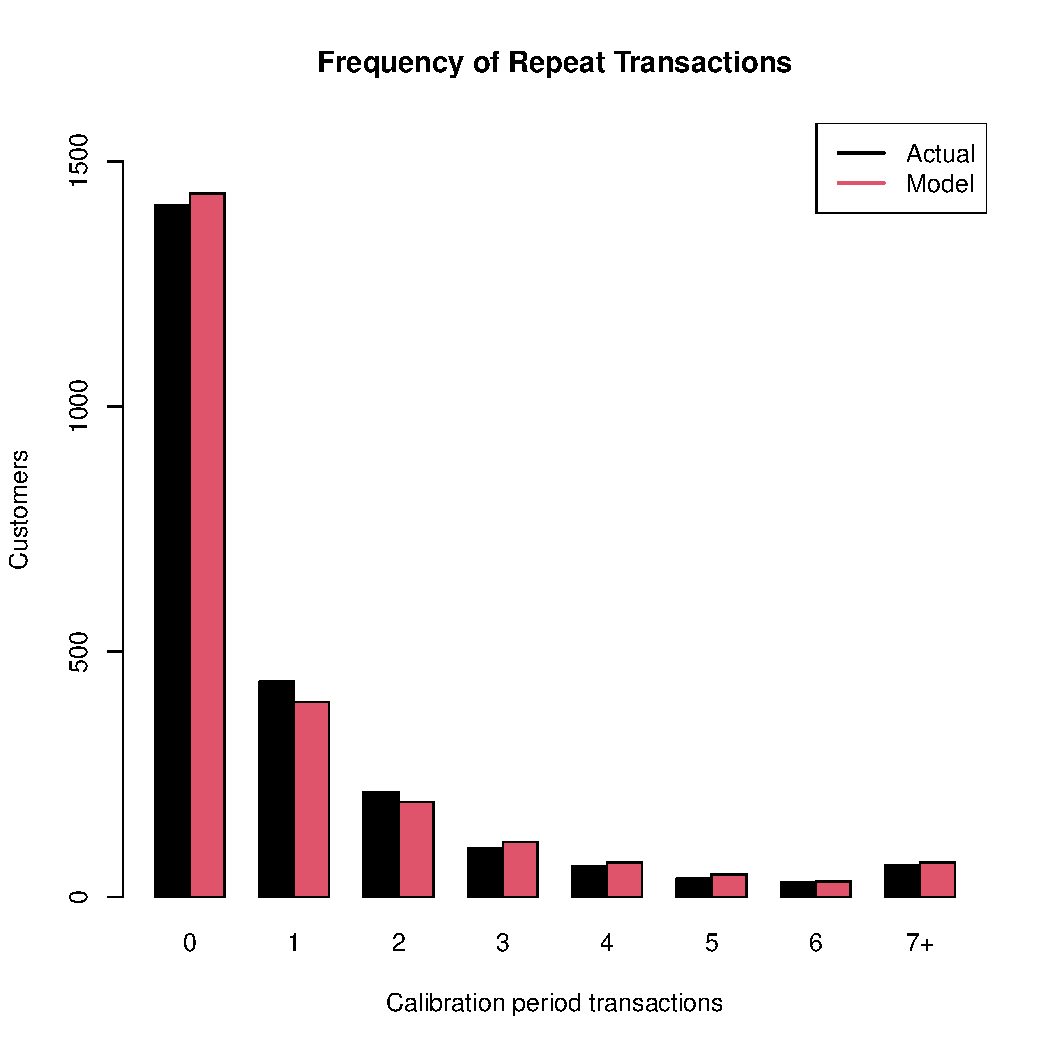
\includegraphics[width=0.6\textwidth]{figure/pnbdCalibrationFit}
  \caption{Calibration period fit of Pareto/NBD model to CDNOW dataset.}\label{fig:pnbdCalibrationFit}
  \end{center}
\end{figure}

\subsection{Data Preparation}

The data required to estimate Pareto/NBD model parameters is
surprisingly little. The customer-by-customer approach of the model is
retained, but we need only three pieces of information for every
person: how many transactions they made in the calibration period
(frequency), the time of their last transaction (recency), and the
total time for which they were observed. A
customer-by-sufficient-statistic matrix, as used by the BTYD package,
is simply a matrix with a row for every customer and a column for each
of the above-mentioned statistics.

You may find yourself with the data available as an event log. This is
a data structure which contains a row for every transaction, with a
customer identifier, date of purchase, and (optionally) the amount of
the transaction. \texttt{dc.ReadLines} is a function to convert an
event log in a comma-delimited file to an data frame in R---you could
use another function such as \texttt{read.csv} or \texttt{read.table}
if desired, but \texttt{dc.ReadLines} simplifies things by only
reading the data you require and giving the output appropriate column
names. In the example below, we create an event log from the file
``cdnowElog.csv'', which has customer IDs in the second column, dates
in the third column and sales numbers in the fifth column.

\begin{knitrout}
\definecolor{shadecolor}{rgb}{0.969, 0.969, 0.969}\color{fgcolor}\begin{kframe}
\begin{alltt}
\hlstd{cdnowElog} \hlkwb{<-} \hlkwd{system.file}\hlstd{(}\hlstr{"data/cdnowElog.csv"}\hlstd{,} \hlkwc{package} \hlstd{=} \hlstr{"BTYD"}\hlstd{)}
\hlstd{elog} \hlkwb{<-} \hlkwd{dc.ReadLines}\hlstd{(cdnowElog,} \hlkwc{cust.idx} \hlstd{=} \hlnum{2}\hlstd{,}
                     \hlkwc{date.idx} \hlstd{=} \hlnum{3}\hlstd{,} \hlkwc{sales.idx} \hlstd{=} \hlnum{5}\hlstd{)}
\hlstd{elog[}\hlnum{1}\hlopt{:}\hlnum{3}\hlstd{,]}
\end{alltt}
\begin{verbatim}
#   cust     date sales
# 1    1 19970101 29.33
# 2    1 19970118 29.73
# 3    1 19970802 14.96
\end{verbatim}
\end{kframe}
\end{knitrout}

Note the formatting of the dates in the output
above. \texttt{dc.Readlines} saves dates as characters, exactly as
they appeared in the original comma-delimited file. For many of the
data-conversion functions in BTYD, however, dates need to be compared
to each other---and unless your years/months/days happen to be in the
right order, you probably want them to be sorted chronologically and not
alphabetically. Therefore, we convert the dates in the event log to R
Date objects:

\begin{knitrout}
\definecolor{shadecolor}{rgb}{0.969, 0.969, 0.969}\color{fgcolor}\begin{kframe}
\begin{alltt}
\hlstd{elog}\hlopt{$}\hlstd{date} \hlkwb{<-} \hlkwd{as.Date}\hlstd{(elog}\hlopt{$}\hlstd{date,} \hlstr{"%Y%m%d"}\hlstd{);}
\hlstd{elog[}\hlnum{1}\hlopt{:}\hlnum{3}\hlstd{,]}
\end{alltt}
\begin{verbatim}
#   cust       date sales
# 1    1 1997-01-01 29.33
# 2    1 1997-01-18 29.73
# 3    1 1997-08-02 14.96
\end{verbatim}
\end{kframe}
\end{knitrout}

Our event log now has dates in the right format, but a bit more
cleaning needs to be done. Transaction-flow models, such as the
Pareto/NBD, is concerned with interpurchase time. Since our timing
information is only accurate to the day, we should merge all
transactions that occurred on the same day. For this, we use
\texttt{dc.MergeTransactionsOnSameDate}. This function returns an
event log with only one transaction per customer per day, with the
total sum of their spending for that day as the sales number. 

\begin{knitrout}
\definecolor{shadecolor}{rgb}{0.969, 0.969, 0.969}\color{fgcolor}\begin{kframe}
\begin{alltt}
\hlstd{elog} \hlkwb{<-} \hlkwd{dc.MergeTransactionsOnSameDate}\hlstd{(elog);}
\end{alltt}
\end{kframe}
\end{knitrout}

To validate that the model works, we need to divide the data up into a
calibration period and a holdout period. This is relatively simple
with either an event log or a customer-by-time matrix, which we are
going to create soon. I am going to use 30 September 1997 as the
cutoff date, as this point (39 weeks) divides the dataset in half. The
reason for doing this split now will become evident when we are
building a customer-by-sufficient-statistic matrix from the
customer-by-time matrix---it requires a last transaction date, and we
want to make sure that last transaction date is the last date in the
calibration period and not in the total period.

\begin{knitrout}
\definecolor{shadecolor}{rgb}{0.969, 0.969, 0.969}\color{fgcolor}\begin{kframe}
\begin{alltt}
\hlstd{end.of.cal.period} \hlkwb{<-} \hlkwd{as.Date}\hlstd{(}\hlstr{"1997-09-30"}\hlstd{)}
\hlstd{elog.cal} \hlkwb{<-} \hlstd{elog[}\hlkwd{which}\hlstd{(elog}\hlopt{$}\hlstd{date} \hlopt{<=} \hlstd{end.of.cal.period), ]}
\end{alltt}
\end{kframe}
\end{knitrout}

The final cleanup step is a very important one. In the calibration
period, the Pareto/NBD model is generally concerned with \emph{repeat}
transactions---that is, the first transaction is ignored. This is
convenient for firms using the model in practice, since it is easier
to keep track of all customers who have made at least one transaction
(as opposed to trying to account for those who have not made any
transactions at all). The one problem with simply getting rid of
customers' first transactions is the following: We have to keep track
of a ``time zero'' as a point of reference for recency and total time
observed. For this reason, we use
\texttt{dc.SplitUpElogForRepeatTrans}, which returns a filtered event
log (\texttt{\$repeat.trans.elog}) as well as saving important
information about each customer (\texttt{\$cust.data}).

\begin{knitrout}
\definecolor{shadecolor}{rgb}{0.969, 0.969, 0.969}\color{fgcolor}\begin{kframe}
\begin{alltt}
\hlstd{split.data} \hlkwb{<-} \hlkwd{dc.SplitUpElogForRepeatTrans}\hlstd{(elog.cal);}
\hlstd{clean.elog} \hlkwb{<-} \hlstd{split.data}\hlopt{$}\hlstd{repeat.trans.elog;}
\end{alltt}
\end{kframe}
\end{knitrout}

The next step is to create a customer-by-time matrix. This is simply a
matrix with a row for each customer and a column for each date. There
are several different options for creating these matrices:
\begin{itemize}
  \item[-] Frequency---each matrix entry will contain the number of
    transactions made by that customer on that day. Use
    \texttt{dc.CreateFreqCBT}. If you have already used
    \texttt{dc.MergeTransactionsOnSameDate}, this will simply be a
    reach customer-by-time matrix.
  \item[-] Reach---each matrix entry will contain a 1 if the customer
    made any transactions on that day, and 0 otherwise. Use
    \texttt{dc.CreateReachCBT}.
  \item[-] Spend---each matrix entry will contain the amount spent by
    that customer on that day. Use \texttt{dc.CreateSpendCBT}. You can
    set whether to use total spend for each day or average spend for
    each day by changing the \texttt{is.avg.spend} parameter. In most
    cases, leaving \texttt{is.avg.spend} as \texttt{FALSE} is appropriate.
\end{itemize}
 
\begin{knitrout}
\definecolor{shadecolor}{rgb}{0.969, 0.969, 0.969}\color{fgcolor}\begin{kframe}
\begin{alltt}
\hlstd{freq.cbt} \hlkwb{<-} \hlkwd{dc.CreateFreqCBT}\hlstd{(clean.elog);}
\hlstd{freq.cbt[}\hlnum{1}\hlopt{:}\hlnum{3}\hlstd{,}\hlnum{1}\hlopt{:}\hlnum{5}\hlstd{]}
\end{alltt}
\begin{verbatim}
#     date
# cust 1997-01-08 1997-01-09 1997-01-10 1997-01-11 1997-01-12
#    1          0          0          0          0          0
#    2          0          0          0          0          0
#    6          0          0          0          1          0
\end{verbatim}
\end{kframe}
\end{knitrout}

There are two things to note from the output above:
\begin{enumerate}
  \item Customers 3, 4, and 5 appear to be missing, and in fact they
    are. They did not make any repeat transactions and were removed
    when we used \texttt{dc.SplitUpElogForRepeatTrans}. Do not worry
    though---we will get them back into the data when we use
    \texttt{dc.MergeCustomers} (soon).
  \item The columns start on January 8---this is because we removed
    all the first transactions (and nobody made 2 transactions withing
    the first week).
\end{enumerate}

We have a small problem now---since we have deleted all the first
transactions, the frequency customer-by-time matrix does not have any
of the customers who made zero repeat transactions. These customers
are still important; in fact, in most datasets, more customers make
zero repeat transactions than any other number. Solving the problem is
reasonably simple: we create a customer-by-time matrix using all
transactions, and then merge the filtered CBT with this total CBT
(using data from the filtered CBT and customer IDs from the total
CBT).

\begin{knitrout}
\definecolor{shadecolor}{rgb}{0.969, 0.969, 0.969}\color{fgcolor}\begin{kframe}
\begin{alltt}
\hlstd{tot.cbt} \hlkwb{<-} \hlkwd{dc.CreateFreqCBT}\hlstd{(elog)}
\hlstd{cal.cbt} \hlkwb{<-} \hlkwd{dc.MergeCustomers}\hlstd{(tot.cbt, freq.cbt)}
\end{alltt}
\end{kframe}
\end{knitrout}

From the calibration period customer-by-time matrix (and a bit of
additional information we saved earlier), we can finally create the
customer-by-sufficient-statistic matrix described earlier. The
function we are going to use is \texttt{dc.BuildCBSFromCBTAndDates},
which requires a customer-by-time matrix, starting and ending dates
for each customer, and the time of the end of the calibration period.
It also requires a time period to use---in this case, we are choosing
to use weeks. If we chose days instead, for example, the recency and
total time observed columns in the customer-by-sufficient-statistic
matrix would have gone up to 273 instead of 39, but it would be the
same data in the end. This function could also be used for the holdout
period by setting \texttt{cbt.is.during.cal.period} to
\texttt{FALSE}. There are slight differences when this function is
used for the holdout period---it requires different input dates
(simply the start and end of the holdout period) and does not return a
recency (which has little value in the holdout period).

\begin{knitrout}
\definecolor{shadecolor}{rgb}{0.969, 0.969, 0.969}\color{fgcolor}\begin{kframe}
\begin{alltt}
\hlstd{birth.periods} \hlkwb{<-} \hlstd{split.data}\hlopt{$}\hlstd{cust.data}\hlopt{$}\hlstd{birth.per}
\hlstd{last.dates} \hlkwb{<-} \hlstd{split.data}\hlopt{$}\hlstd{cust.data}\hlopt{$}\hlstd{last.date}
\hlstd{cal.cbs.dates} \hlkwb{<-} \hlkwd{data.frame}\hlstd{(birth.periods, last.dates,}
                            \hlstd{end.of.cal.period)}
\hlstd{cal.cbs} \hlkwb{<-} \hlkwd{dc.BuildCBSFromCBTAndDates}\hlstd{(cal.cbt, cal.cbs.dates,}
                                      \hlkwc{per}\hlstd{=}\hlstr{"week"}\hlstd{)}
\end{alltt}
\end{kframe}
\end{knitrout}

You'll be glad to hear that, for the process described above, the
package contains a single function to do everything for you:
\texttt{dc.ElogToCbsCbt}. However, it is good to be aware of the
process above, as you might want to make small changes for different
situations---for example, you may not want to remove customers'
initial transactions, or your data may be available as a
customer-by-time matrix and not as an event log. For most standard
situations, however, \texttt{dc.ElogToCbsCbt} will do. Reading about
its parameters and output in the package documentation will help you
to understand the function well enough to use it for most purposes.

\subsection{Parameter Estimation}

Now that we have the data in the correct format, we can estimate model
parameters. To estimate parameters, we use
\texttt{pnbd.EstimateParameters}, which requires a calibration period
customer-by-sufficient-statistic matrix and (optionally) starting
parameters. (1,1,1,1) is used as default starting parameters if none
are provided. The function which is maximized is \texttt{pnbd.cbs.LL},
which returns the log-likelihood of a given set of parameters for a
customer-by-sufficient-statistic matrix.

\begin{knitrout}
\definecolor{shadecolor}{rgb}{0.969, 0.969, 0.969}\color{fgcolor}\begin{kframe}
\begin{alltt}
\hlstd{params} \hlkwb{<-} \hlkwd{pnbd.EstimateParameters}\hlstd{(}\hlkwc{cal.cbs} \hlstd{= cal.cbs,}
                                  \hlkwc{hardie} \hlstd{= allHardie);}
\hlkwd{round}\hlstd{(params,} \hlkwc{digits} \hlstd{=} \hlnum{3}\hlstd{)}
\end{alltt}
\begin{verbatim}
# [1]  0.553 10.580  0.606 11.656
\end{verbatim}
\begin{alltt}
\hlstd{LL} \hlkwb{<-} \hlkwd{pnbd.cbs.LL}\hlstd{(}\hlkwc{params} \hlstd{= params,}
                  \hlkwc{cal.cbs} \hlstd{= cal.cbs,}
                  \hlkwc{hardie} \hlstd{= allHardie)}
\hlstd{LL}
\end{alltt}
\begin{verbatim}
# [1] -9594.976
\end{verbatim}
\end{kframe}
\end{knitrout}

As with any optimization, we should not be satisfied with the first
output we get. Let's run it a couple more times, with its own output
as a starting point, to see if it converges:

\begin{knitrout}
\definecolor{shadecolor}{rgb}{0.969, 0.969, 0.969}\color{fgcolor}\begin{kframe}
\begin{alltt}
\hlstd{p.matrix} \hlkwb{<-} \hlkwd{c}\hlstd{(params, LL)}
\hlkwa{for} \hlstd{(i} \hlkwa{in} \hlnum{1}\hlopt{:}\hlnum{2}\hlstd{)\{}
  \hlstd{params} \hlkwb{<-} \hlkwd{pnbd.EstimateParameters}\hlstd{(}\hlkwc{cal.cbs} \hlstd{= cal.cbs,}
                                    \hlkwc{par.start} \hlstd{= params,}
                                    \hlkwc{hardie} \hlstd{= allHardie)}
  \hlstd{LL} \hlkwb{<-} \hlkwd{pnbd.cbs.LL}\hlstd{(}\hlkwc{params} \hlstd{= params,}
                    \hlkwc{cal.cbs} \hlstd{= cal.cbs,}
                    \hlkwc{hardie} \hlstd{= allHardie)}
  \hlstd{p.matrix.row} \hlkwb{<-} \hlkwd{c}\hlstd{(params, LL)}
  \hlstd{p.matrix} \hlkwb{<-} \hlkwd{rbind}\hlstd{(p.matrix, p.matrix.row)}
\hlstd{\}}
\hlkwd{colnames}\hlstd{(p.matrix)} \hlkwb{<-} \hlkwd{c}\hlstd{(}\hlstr{"r"}\hlstd{,} \hlstr{"alpha"}\hlstd{,} \hlstr{"s"}\hlstd{,} \hlstr{"beta"}\hlstd{,} \hlstr{"LL"}\hlstd{)}
\hlkwd{rownames}\hlstd{(p.matrix)} \hlkwb{<-} \hlnum{1}\hlopt{:}\hlnum{3}
\hlkwd{round}\hlstd{(p.matrix,} \hlkwc{digits} \hlstd{=} \hlnum{3}\hlstd{)}
\end{alltt}
\begin{verbatim}
#       r alpha     s   beta        LL
# 1 0.553 10.58 0.606 11.656 -9594.976
# 2 0.553 10.58 0.606 11.657 -9594.976
# 3 0.553 10.58 0.606 11.658 -9594.976
\end{verbatim}
\end{kframe}
\end{knitrout}

This estimation does converge. I am not going to demonstrate it here,
but it is always a good idea to test the estimation function
from several starting points.

Now that we have the parameters, the BTYD package provides functions
to interpret them. As we know, r and alpha describe the gamma mixing
distribution of the NBD transaction process. We can see this gamma
distribution in figure \ref{fig:pnbdTransactionHeterogeneity}, plotted
using \texttt{pnbd.PlotTransactionRateHeterogeneity(params)}. We also
know that s and beta describe the gamma mixing distribution of the
Pareto (or gamma exponential) dropout process. We can see this gamma
distribution in figure \ref{fig:pnbdDropoutHeterogeneity}, plotted
using \texttt{pnbd.PlotDropoutRateHeterogeneity(params)}.

From these, we can already tell something about our customers: they
are more likely to have low values for their individual poisson
transaction process parameters, and more likely to have low values for
their individual exponential dropout process parameters.



\begin{figure}
  \begin{center}
  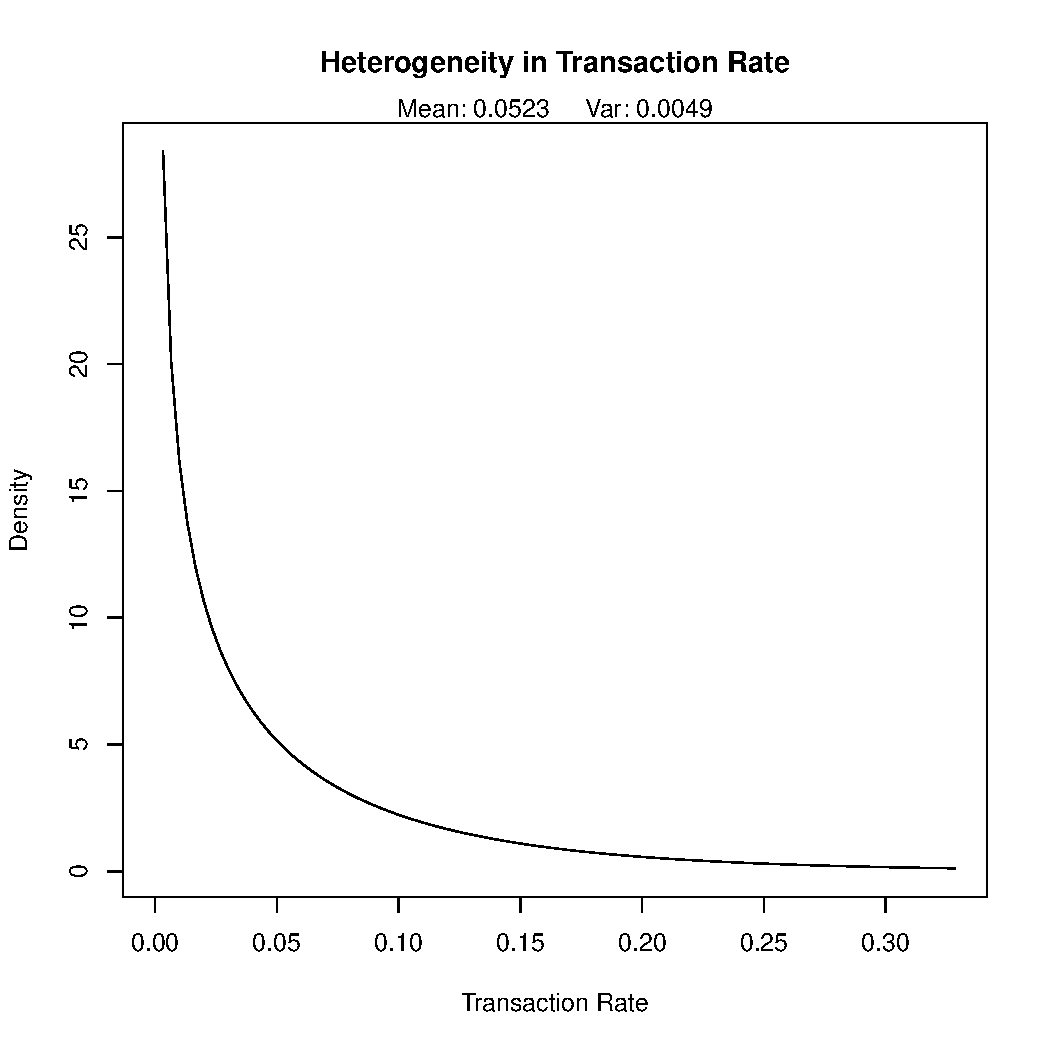
\includegraphics[width=0.6\textwidth]{figure/pnbdTransactionHeterogeneity}
  \caption{Transaction rate heterogeneity of estimated parameters.}\label{fig:pnbdTransactionHeterogeneity}
  \end{center}
\end{figure}



\begin{figure}
  \begin{center}
  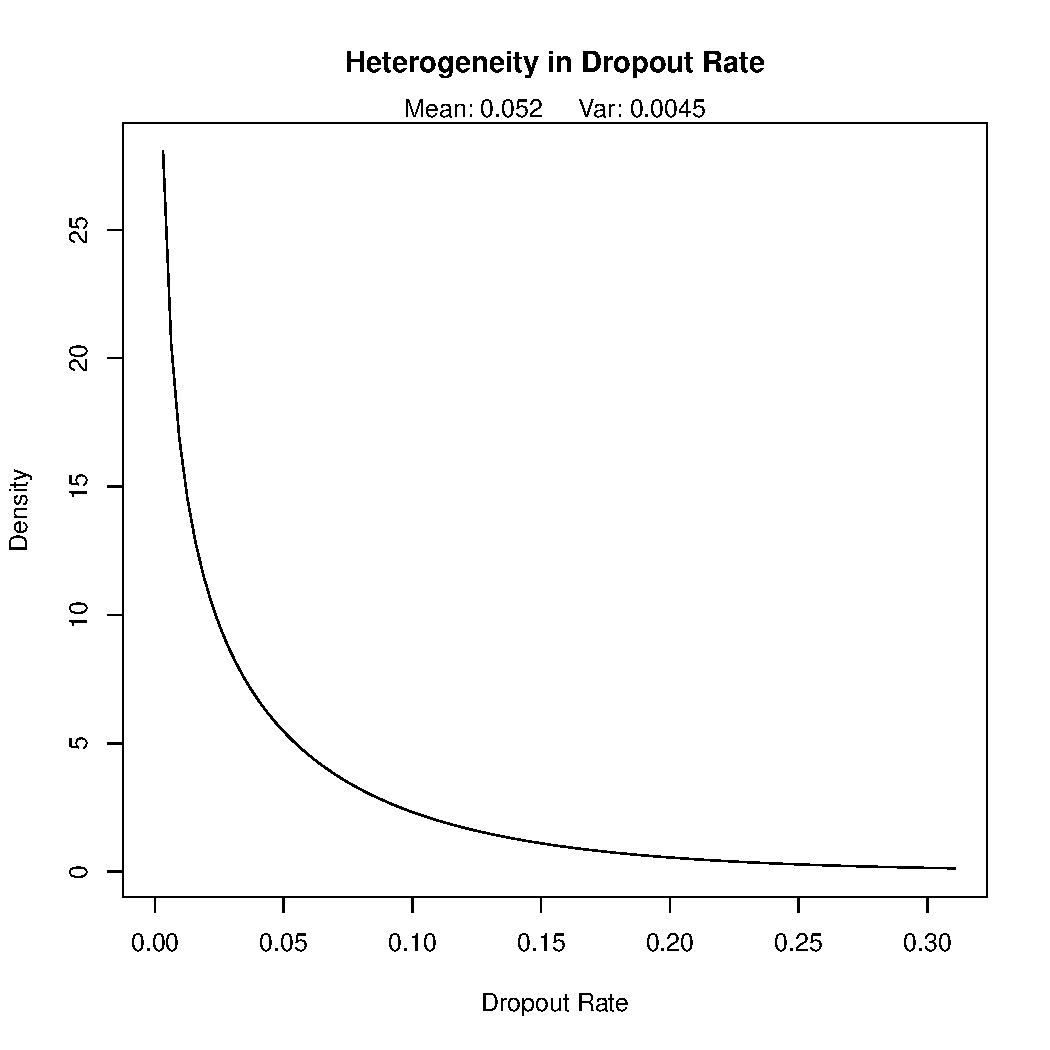
\includegraphics[width=0.6\textwidth]{figure/pnbdDropoutHeterogeneity}
  \caption{Dropout rate heterogeneity of estimated parameters.}\label{fig:pnbdDropoutHeterogeneity}
  \end{center}
\end{figure}
 
\subsection{Individual Level Estimations}
Now that we have parameters for the population, we can make
estimations for customers on the individual level.

First, we can estimate the number of transactions we expect a newly
acquired customer to make in a given time period. Let's say, for
example, that we are interested in the number of repeat transactions a
newly acquired customer will make in a time period of one year. Note
that we use 52 weeks to represent one year, not 12 months, 365 days,
or 1 year. This is because our parameters were estimated using weekly
data.

\begin{knitrout}
\definecolor{shadecolor}{rgb}{0.969, 0.969, 0.969}\color{fgcolor}\begin{kframe}
\begin{alltt}
\hlkwd{pnbd.Expectation}\hlstd{(}\hlkwc{params} \hlstd{= params,} \hlkwc{t} \hlstd{=} \hlnum{52}\hlstd{)}
\end{alltt}
\begin{verbatim}
# [1] 1.473434
\end{verbatim}
\end{kframe}
\end{knitrout}

We can also obtain expected characteristics for a specific customer,
conditional on their purchasing behavior during the calibration
period. The first of these is
\texttt{pnbd.ConditionalExpectedTransactions}, which gives the number
of transactions we expect a customer to make in the holdout
period. The second is \texttt{pnbd.PAlive}, which gives the
probability that a customer is still alive at the end of the
calibration period. As above, the time periods used depend on which
time period was used to estimate the parameters. 

\begin{knitrout}
\definecolor{shadecolor}{rgb}{0.969, 0.969, 0.969}\color{fgcolor}\begin{kframe}
\begin{alltt}
\hlstd{cal.cbs[}\hlstr{"1516"}\hlstd{,]}
\end{alltt}
\begin{verbatim}
#        x      t.x    T.cal 
# 26.00000 30.85714 31.00000
\end{verbatim}
\begin{alltt}
\hlstd{x} \hlkwb{<-} \hlstd{cal.cbs[}\hlstr{"1516"}\hlstd{,} \hlstr{"x"}\hlstd{]}
\hlstd{t.x} \hlkwb{<-} \hlstd{cal.cbs[}\hlstr{"1516"}\hlstd{,} \hlstr{"t.x"}\hlstd{]}
\hlstd{T.cal} \hlkwb{<-} \hlstd{cal.cbs[}\hlstr{"1516"}\hlstd{,} \hlstr{"T.cal"}\hlstd{]}
\hlkwd{pnbd.ConditionalExpectedTransactions}\hlstd{(params,}
                                     \hlkwc{T.star} \hlstd{=} \hlnum{52}\hlstd{,}
                                     \hlstd{x,}
                                     \hlstd{t.x,}
                                     \hlstd{T.cal,}
                                     \hlkwc{hardie} \hlstd{= allHardie)}
\end{alltt}
\begin{verbatim}
# [1] 25.45647
\end{verbatim}
\begin{alltt}
\hlkwd{pnbd.PAlive}\hlstd{(params,}
            \hlstd{x,}
            \hlstd{t.x,}
            \hlstd{T.cal,}
            \hlkwc{hardie} \hlstd{= allHardie)}
\end{alltt}
\begin{verbatim}
# [1] 0.997874
\end{verbatim}
\end{kframe}
\end{knitrout}

There is one more point to note here---using the conditional
expectation function, we can see the ``increasing frequency paradox''
in action:

\begin{knitrout}
\definecolor{shadecolor}{rgb}{0.969, 0.969, 0.969}\color{fgcolor}\begin{kframe}
\begin{alltt}
\hlcom{# avoid overflow in LaTeX code block here:}
\hlstd{cet} \hlkwb{<-} \hlstr{"pnbd.ConditionalExpectedTransactions"}
\hlkwa{for} \hlstd{(i} \hlkwa{in} \hlkwd{seq}\hlstd{(}\hlnum{10}\hlstd{,} \hlnum{25}\hlstd{,} \hlnum{5}\hlstd{))\{}
  \hlstd{cond.expectation} \hlkwb{<-} \hlkwd{match.fun}\hlstd{(cet)(params,}
                                     \hlkwc{T.star} \hlstd{=} \hlnum{52}\hlstd{,}
                                     \hlkwc{x} \hlstd{= i,}
                                     \hlkwc{t.x} \hlstd{=} \hlnum{20}\hlstd{,}
                                     \hlkwc{T.cal} \hlstd{=} \hlnum{39}\hlstd{,}
                                     \hlkwc{hardie} \hlstd{= allHardie)}
  \hlkwd{cat} \hlstd{(}\hlstr{"x:"}\hlstd{,i,}\hlstr{"\textbackslash{}t Expectation:"}\hlstd{,cond.expectation,} \hlkwc{fill} \hlstd{=} \hlnum{TRUE}\hlstd{)}
\hlstd{\}}
\end{alltt}
\begin{verbatim}
# x: 10 	 Expectation: 0.7062289
# x: 15 	 Expectation: 0.1442396
# x: 20 	 Expectation: 0.02250658
# x: 25 	 Expectation: 0.00309267
\end{verbatim}
\end{kframe}
\end{knitrout}

\subsection{Plotting/ Goodness-of-fit}
\label{subsec:pnbdPlotting}
We would like to be able to do more than make inferences about
individual customers. The BTYD package provides functions to plot
expected customer behavior against actual customer behavior in the
both the calibration and holdout periods.

The first such function is the obvious starting point: a comparison of
actual and expected frequencies within the calibration period. This is
figure \ref{fig:pnbdCalibrationFit}, which was generated using the
following code:

\begin{knitrout}
\definecolor{shadecolor}{rgb}{0.969, 0.969, 0.969}\color{fgcolor}\begin{kframe}
\begin{alltt}
\hlkwd{pnbd.PlotFrequencyInCalibration}\hlstd{(}\hlkwc{params} \hlstd{= params,}
                                \hlkwc{cal.cbs} \hlstd{= cal.cbs,}
                                \hlkwc{censor} \hlstd{=} \hlnum{7}\hlstd{,}
                                \hlkwc{hardie} \hlstd{= allHardie)}
\end{alltt}
\end{kframe}
\end{knitrout}

This function obviously needs to be able to generate expected data
(from estimated parameters) and requires the actual data (the
calibration period customer-by-sufficient-statistic).  It also
requires another number, called the censor number. The histogram that
is plotted is right-censored; after a certain number, all frequencies
are binned together. The number provided as a censor number determines
where the data is cut off.

Unfortunately, the only thing we can tell from comparing calibration
period frequencies is that the fit between our model and the data
isn't awful. We need to verify that the fit of the model holds into
the holdout period. Firstly, however, we are are going to need to get
information for holdout period. \texttt{dc.ElogToCbsCbt} produces both
a calibration period customer-by-sufficient-statistic matrix and a
holdout period customer-by-sufficient-statistic matrix, which could be
combined in order to find the number of transactions each customer
made in the holdout period. However, since we did not use
\texttt{dc.ElogToCbsCbt}, I am going to get the information directly
from the event log. Note that I subtract the number of repeat
transactions in the calibration period from the total number of
transactions. We remove the initial transactions first as we are not
concerned with them.

\begin{knitrout}
\definecolor{shadecolor}{rgb}{0.969, 0.969, 0.969}\color{fgcolor}\begin{kframe}
\begin{alltt}
\hlstd{elog} \hlkwb{<-} \hlkwd{dc.SplitUpElogForRepeatTrans}\hlstd{(elog)}\hlopt{$}\hlstd{repeat.trans.elog;}
\hlstd{x.star} \hlkwb{<-} \hlkwd{rep}\hlstd{(}\hlnum{0}\hlstd{,} \hlkwd{nrow}\hlstd{(cal.cbs));}
\hlstd{cal.cbs} \hlkwb{<-} \hlkwd{cbind}\hlstd{(cal.cbs, x.star);}
\hlstd{elog.custs} \hlkwb{<-} \hlstd{elog}\hlopt{$}\hlstd{cust;}
\hlkwa{for} \hlstd{(i} \hlkwa{in} \hlnum{1}\hlopt{:}\hlkwd{nrow}\hlstd{(cal.cbs))\{}
  \hlstd{current.cust} \hlkwb{<-} \hlkwd{rownames}\hlstd{(cal.cbs)[i]}
  \hlstd{tot.cust.trans} \hlkwb{<-} \hlkwd{length}\hlstd{(}\hlkwd{which}\hlstd{(elog.custs} \hlopt{==} \hlstd{current.cust))}
  \hlstd{cal.trans} \hlkwb{<-} \hlstd{cal.cbs[i,} \hlstr{"x"}\hlstd{]}
  \hlstd{cal.cbs[i,} \hlstr{"x.star"}\hlstd{]} \hlkwb{<-}  \hlstd{tot.cust.trans} \hlopt{-} \hlstd{cal.trans}
\hlstd{\}}
\hlkwd{round}\hlstd{(cal.cbs[}\hlnum{1}\hlopt{:}\hlnum{3}\hlstd{,],} \hlkwc{digits} \hlstd{=} \hlnum{3}\hlstd{)}
\end{alltt}
\begin{verbatim}
#   x    t.x  T.cal x.star
# 1 2 30.429 38.857      1
# 2 1  1.714 38.857      0
# 3 0  0.000 38.857      0
\end{verbatim}
\end{kframe}
\end{knitrout}

Now we can see how well our model does in the holdout period. Figure
\ref{fig:pnbdCondExpComp} shows the output produced by the code below. It
divides the customers up into bins according to calibration period
frequencies and plots actual and conditional expected holdout period
frequencies for these bins.

\begin{knitrout}\small
\definecolor{shadecolor}{rgb}{0.969, 0.969, 0.969}\color{fgcolor}\begin{kframe}
\begin{alltt}
\hlstd{T.star} \hlkwb{<-} \hlnum{39} \hlcom{# length of the holdout period}
\hlstd{censor} \hlkwb{<-} \hlnum{7}  \hlcom{# This censor serves the same purpose described above}
\hlstd{x.star} \hlkwb{<-} \hlstd{cal.cbs[,}\hlstr{"x.star"}\hlstd{]}
\hlkwd{pdf}\hlstd{(}\hlkwc{file} \hlstd{=} \hlstr{'figure/pnbdCondExpComp.pdf'}\hlstd{)}
\hlstd{comp} \hlkwb{<-} \hlkwd{pnbd.PlotFreqVsConditionalExpectedFrequency}\hlstd{(params,}
                                                    \hlstd{T.star,}
                                                    \hlstd{cal.cbs,}
                                                    \hlstd{x.star,}
                                                    \hlstd{censor,}
                                                    \hlkwc{hardie} \hlstd{= allHardie)}
\hlkwd{dev.off}\hlstd{()}
\end{alltt}
\begin{verbatim}
# pdf 
#   2
\end{verbatim}
\begin{alltt}
\hlkwd{rownames}\hlstd{(comp)} \hlkwb{<-} \hlkwd{c}\hlstd{(}\hlstr{"act"}\hlstd{,} \hlstr{"exp"}\hlstd{,} \hlstr{"bin"}\hlstd{)}
\hlkwd{round}\hlstd{(comp,} \hlkwc{digits} \hlstd{=} \hlnum{3}\hlstd{)}
\end{alltt}
\begin{verbatim}
#       freq.0  freq.1  freq.2  freq.3 freq.4 freq.5 freq.6 freq.7+
# act    0.237   0.697   1.393   1.560  2.532  2.947  3.862   6.359
# exp    0.138   0.600   1.196   1.714  2.399  2.907  3.819   6.403
# bin 1411.000 439.000 214.000 100.000 62.000 38.000 29.000  64.000
\end{verbatim}
\end{kframe}
\end{knitrout}

\begin{figure}
  \begin{center}
  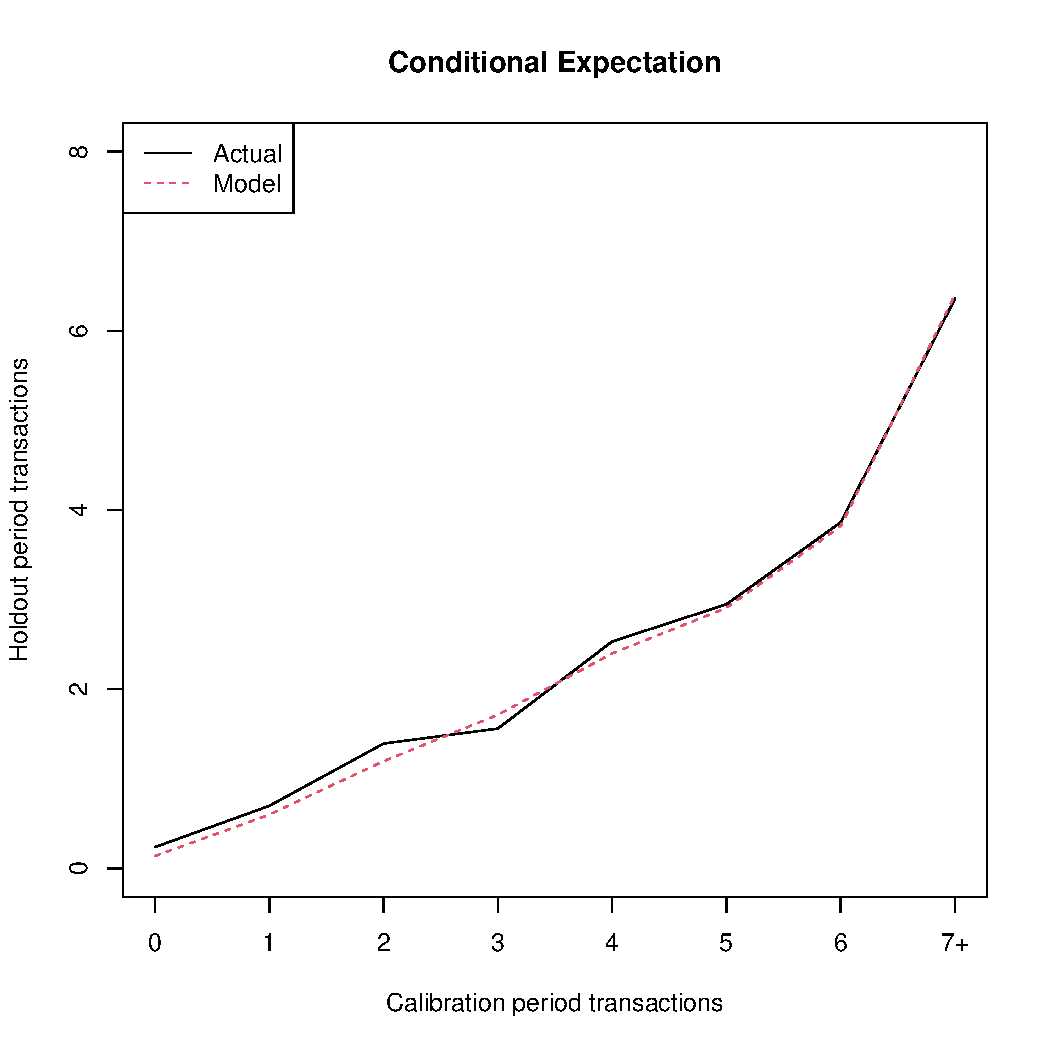
\includegraphics[width=0.6\textwidth]{figure/pnbdCondExpComp}
  \caption{Actual vs. conditional expected transactions in the holdout period.}\label{fig:pnbdCondExpComp}
  \end{center}
\end{figure}

As you can see above, the graph also produces a matrix output. Most
plotting functions in the BTYD package produce output like this. They
are often worth looking at because they contain additional information
not presented in the graph---the size of each bin in the graph. In
this graph, for example, this information is important because the bin
sizes show that the gap at zero means a lot more than the precision at
6 or 7 transactions. Despite this, this graph shows that the model
fits the data very well in the holdout period.

Aggregation by calibration period frequency is just one way to do
it. BTYD also provides plotting functions which aggregate by several
other measures. The other one I will demonstrate here is aggregation
by time---how well does our model predict how many transactions will
occur in each week?

The first step, once again, is going to be to collect the data we need
to compare the model to. The customer-by-time matrix has already
collected the data for us by time period; so we'll use that to gather
the total transactions per day. Then we convert the daily tracking
data to weekly data.

\begin{knitrout}
\definecolor{shadecolor}{rgb}{0.969, 0.969, 0.969}\color{fgcolor}\begin{kframe}
\begin{alltt}
\hlstd{tot.cbt} \hlkwb{<-} \hlkwd{dc.CreateFreqCBT}\hlstd{(elog)}
\end{alltt}


{\ttfamily\noindent\itshape\color{messagecolor}{\# ...Completed Freq CBT}}\begin{alltt}
\hlstd{d.track.data} \hlkwb{<-} \hlkwd{rep}\hlstd{(}\hlnum{0}\hlstd{,} \hlnum{7} \hlopt{*} \hlnum{78}\hlstd{)}
\hlstd{origin} \hlkwb{<-} \hlkwd{as.Date}\hlstd{(}\hlstr{"1997-01-01"}\hlstd{)}
\hlkwa{for} \hlstd{(i} \hlkwa{in} \hlkwd{colnames}\hlstd{(tot.cbt))\{}
  \hlstd{date.index} \hlkwb{<-} \hlkwd{difftime}\hlstd{(}\hlkwd{as.Date}\hlstd{(i), origin)} \hlopt{+} \hlnum{1}\hlstd{;}
  \hlstd{d.track.data[date.index]} \hlkwb{<-} \hlkwd{sum}\hlstd{(tot.cbt[,i]);}
\hlstd{\}}
\hlstd{w.track.data} \hlkwb{<-}  \hlkwd{rep}\hlstd{(}\hlnum{0}\hlstd{,} \hlnum{78}\hlstd{)}
\hlkwa{for} \hlstd{(j} \hlkwa{in} \hlnum{1}\hlopt{:}\hlnum{78}\hlstd{)\{}
  \hlstd{w.track.data[j]} \hlkwb{<-} \hlkwd{sum}\hlstd{(d.track.data[(j}\hlopt{*}\hlnum{7}\hlopt{-}\hlnum{6}\hlstd{)}\hlopt{:}\hlstd{(j}\hlopt{*}\hlnum{7}\hlstd{)])}
\hlstd{\}}
\end{alltt}
\end{kframe}
\end{knitrout}

Now, we can make a plot comparing the actual number of transactions to
the expected number of transactions on a weekly basis, as shown in
figure \ref{fig:pnbdTrackingInc}. Note that we set
\texttt{n.periods.final} to 78. This is to show that we are working
with weekly data. If our tracking data was daily, we would use 546
here---the function would plot our daily tracking data against
expected daily transactions, instead of plotting our weekly tracking
data against expected weekly transactions. This concept may be a bit
tricky, but is explained in the documentation for
\texttt{pnbd.PlotTrackingInc}. The reason there are two numbers for
the total period (\texttt{T.tot} and \texttt{n.periods.final}) is that
your customer-by-sufficient-statistic matrix and your tracking data
may be in different time periods.

\begin{knitrout}
\definecolor{shadecolor}{rgb}{0.969, 0.969, 0.969}\color{fgcolor}\begin{kframe}
\begin{alltt}
\hlstd{T.cal} \hlkwb{<-} \hlstd{cal.cbs[,}\hlstr{"T.cal"}\hlstd{]}
\hlstd{T.tot} \hlkwb{<-} \hlnum{78}
\hlstd{n.periods.final} \hlkwb{<-} \hlnum{78}

\hlkwd{pdf}\hlstd{(}\hlkwc{file} \hlstd{=} \hlstr{'figure/pnbdTrackingInc.pdf'}\hlstd{)}
\hlstd{inc.tracking} \hlkwb{<-} \hlkwd{pnbd.PlotTrackingInc}\hlstd{(}\hlkwc{params} \hlstd{= params,}
                                     \hlkwc{T.cal} \hlstd{= T.cal,}
                                     \hlkwc{T.tot} \hlstd{= T.tot,}
                                     \hlkwc{actual.inc.tracking.data} \hlstd{= w.track.data,}
                                     \hlkwc{n.periods.final} \hlstd{= n.periods.final)}
\end{alltt}


{\ttfamily\noindent\color{warningcolor}{\# Warning in FUN(X[[i]], ...): Maximum vector length not a multiple of the length of actual.inc.tracking.data}}\begin{alltt}
\hlkwd{dev.off}\hlstd{()}
\end{alltt}
\begin{verbatim}
# pdf 
#   2
\end{verbatim}
\begin{alltt}
\hlkwd{round}\hlstd{(inc.tracking[,}\hlnum{20}\hlopt{:}\hlnum{25}\hlstd{],} \hlkwc{digits} \hlstd{=} \hlnum{3}\hlstd{)}
\end{alltt}
\begin{verbatim}
#            [,1]   [,2]   [,3]   [,4]   [,5]   [,6]
# actual   73.000 55.000 70.000 33.000 56.000 99.000
# expected 78.308 76.419 74.648 72.983 71.414 69.933
\end{verbatim}
\end{kframe}
\end{knitrout}

\begin{figure}
  \begin{center}
  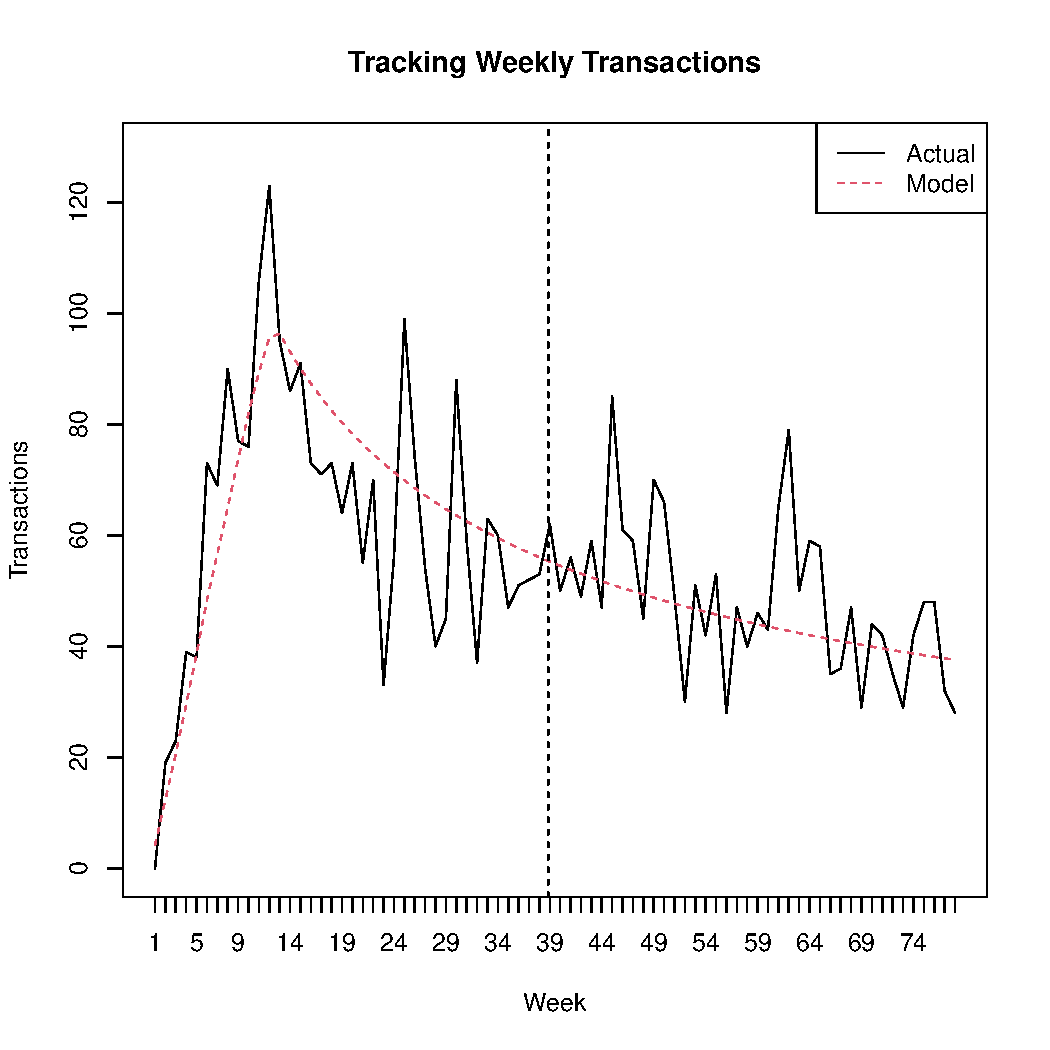
\includegraphics[width=0.6\textwidth]{figure/pnbdTrackingInc}
  \caption{Actual vs. expected incremental purchasing behaviour.}\label{fig:pnbdTrackingInc}
  \end{center}
\end{figure}

Although figure \ref{fig:pnbdTrackingInc} shows that the model is
definitely capturing the trend of customer purchases over time, it is
very messy and may not convince skeptics. Furthermore, the matrix, of
which a sample is shown, does not really convey much information since
purchases can vary so much from one week to the next. For these
reasons, we may need to smooth the data out by cummulating it over
time, as shown in figure \ref{fig:pnbdTrackingCum}.



\begin{knitrout}
\definecolor{shadecolor}{rgb}{0.969, 0.969, 0.969}\color{fgcolor}\begin{kframe}
\begin{alltt}
\hlstd{cum.tracking.data} \hlkwb{<-} \hlkwd{cumsum}\hlstd{(w.track.data)}
\hlkwd{pdf}\hlstd{(}\hlkwc{file} \hlstd{=} \hlstr{'figure/pnbdTrackingCum.pdf'}\hlstd{)}
\hlstd{cum.tracking} \hlkwb{<-} \hlkwd{pnbd.PlotTrackingCum}\hlstd{(}\hlkwc{params} \hlstd{= params,}
                                     \hlkwc{T.cal} \hlstd{= T.cal,}
                                     \hlkwc{T.tot} \hlstd{= T.tot,}
                                     \hlkwc{actual.cu.tracking.data} \hlstd{= cum.tracking.data,}
                                     \hlkwc{n.periods.final} \hlstd{= n.periods.final)}
\end{alltt}


{\ttfamily\noindent\color{warningcolor}{\# Warning in FUN(X[[i]], ...): Maximum vector length not a multiple of the length of actual.cu.tracking.data}}\begin{alltt}
\hlkwd{dev.off}\hlstd{()}
\end{alltt}
\begin{verbatim}
# pdf 
#   2
\end{verbatim}
\begin{alltt}
\hlkwd{round}\hlstd{(cum.tracking[,}\hlnum{20}\hlopt{:}\hlnum{25}\hlstd{],} \hlkwc{digits} \hlstd{=} \hlnum{3}\hlstd{)}
\end{alltt}
\begin{verbatim}
#              [,1]     [,2]     [,3]     [,4]    [,5]     [,6]
# actual   1359.000 1414.000 1484.000 1517.000 1573.00 1672.000
# expected 1308.856 1385.275 1459.923 1532.906 1604.32 1674.253
\end{verbatim}
\end{kframe}
\end{knitrout}

\begin{figure}
  \begin{center}
  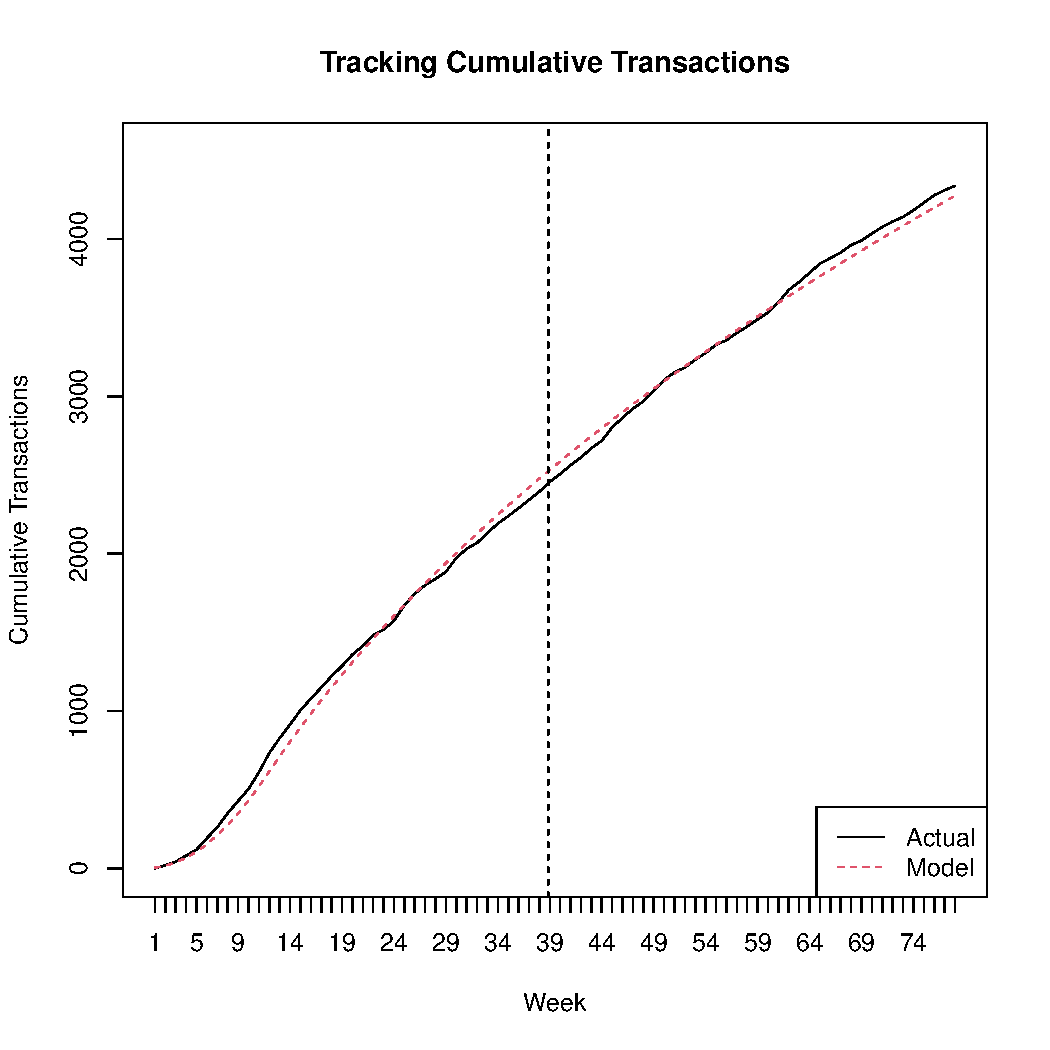
\includegraphics[width=0.6\textwidth]{figure/pnbdTrackingCum}
  \caption{Actual vs. expected cumulative purchasing behaviour.}\label{fig:pnbdTrackingCum}
  \end{center}
\end{figure}









\section{BG/NBD}

The BG/NBD model, like the Pareto/NBD model, is used for non-contractual 
situations in which customers can make purchases at any time. It
describes the rate at which customers make purchases and the rate at
which they drop out with four parameters---allowing for heterogeneity in both. 
We will walk through the BG/NBD functions provided by the BTYD package using the 
CDNOW\footnote{Provided with
  the BTYD package and available at
  \href{http://www.brucehardie.com}{brucehardie.com}. For more
  details, see the documentation of the cdnowSummary data included in
  the package.} dataset. As shown by
figure \ref{fig:bgnbdCalibrationFit}, the BG/NBD model describes
this dataset quite well.



\begin{figure}
  \begin{center}
  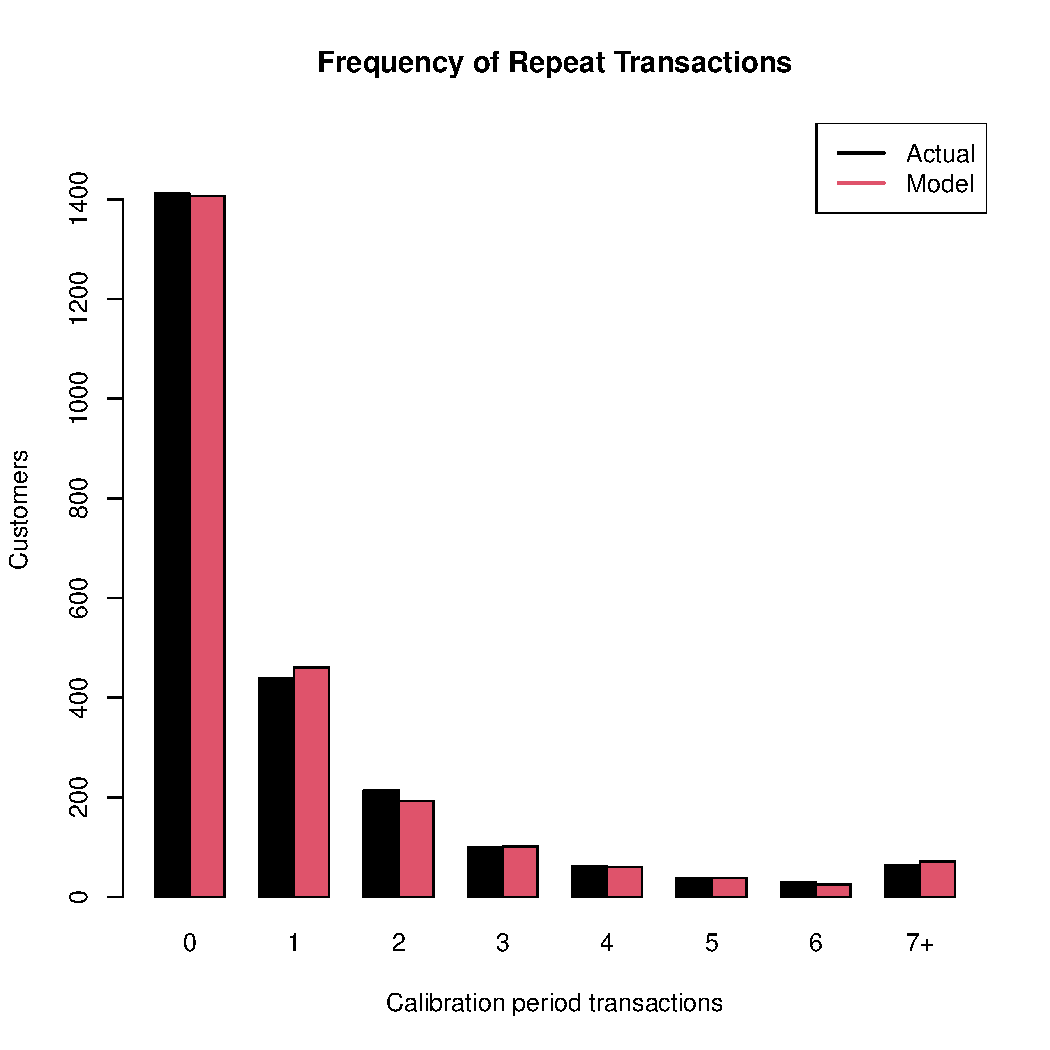
\includegraphics[width=0.6\textwidth]{figure/bgnbdCalibrationFit}
  \caption{Calibration period fit of BG/NBD model to CDNOW dataset.}\label{fig:bgnbdCalibrationFit}
  \end{center}
\end{figure}



\subsection{Data Preparation}

The data required to estimate BG/NBD model parameters is
surprisingly little. The customer-by-customer approach of the model is
retained, but we need only three pieces of information for every
person: how many transactions they made in the calibration period
(frequency), the time of their last transaction (recency), and the
total time for which they were observed. This is the same as what is 
needed for the Pareto/NBD model. Indeed, if you have read the data 
preparation section for the Pareto/NBD model, you can safely skip over
this section and move to the section on Parameter Estimation.  

A customer-by-sufficient-statistic matrix, as used by the BTYD package,
is simply a matrix with a row for every customer and a column for each
of the above-mentioned statistics.

You may find yourself with the data available as an event log. This is
a data structure which contains a row for every transaction, with a
customer identifier, date of purchase, and (optionally) the amount of
the transaction. \texttt{dc.ReadLines} is a function to convert an
event log in a comma-delimited file to an data frame in R---you could
use another function such as \texttt{read.csv} or \texttt{read.table}
if desired, but \texttt{dc.ReadLines} simplifies things by only
reading the data you require and giving the output appropriate column
names. In the example below, we create an event log from the file
``cdnowElog.csv'', which has customer IDs in the second column, dates
in the third column and sales numbers in the fifth column.

\begin{knitrout}
\definecolor{shadecolor}{rgb}{0.969, 0.969, 0.969}\color{fgcolor}\begin{kframe}
\begin{alltt}
\hlstd{cdnowElog} \hlkwb{<-} \hlkwd{system.file}\hlstd{(}\hlstr{"data/cdnowElog.csv"}\hlstd{,} \hlkwc{package} \hlstd{=} \hlstr{"BTYD"}\hlstd{)}
\hlstd{elog} \hlkwb{<-} \hlkwd{dc.ReadLines}\hlstd{(cdnowElog,} \hlkwc{cust.idx} \hlstd{=} \hlnum{2}\hlstd{,}
                     \hlkwc{date.idx} \hlstd{=} \hlnum{3}\hlstd{,} \hlkwc{sales.idx} \hlstd{=} \hlnum{5}\hlstd{)}
\hlstd{elog[}\hlnum{1}\hlopt{:}\hlnum{3}\hlstd{,]}
\end{alltt}
\begin{verbatim}
#   cust     date sales
# 1    1 19970101 29.33
# 2    1 19970118 29.73
# 3    1 19970802 14.96
\end{verbatim}
\end{kframe}
\end{knitrout}

Note the formatting of the dates in the output
above. \texttt{dc.Readlines} saves dates as characters, exactly as
they appeared in the original comma-delimited file. For many of the
data-conversion functions in BTYD, however, dates need to be compared
to each other---and unless your years/months/days happen to be in the
right order, you probably want them to be sorted chronologically and not
alphabetically. Therefore, we convert the dates in the event log to R
Date objects:

\begin{knitrout}
\definecolor{shadecolor}{rgb}{0.969, 0.969, 0.969}\color{fgcolor}\begin{kframe}
\begin{alltt}
\hlstd{elog}\hlopt{$}\hlstd{date} \hlkwb{<-} \hlkwd{as.Date}\hlstd{(elog}\hlopt{$}\hlstd{date,} \hlstr{"%Y%m%d"}\hlstd{);}
\hlstd{elog[}\hlnum{1}\hlopt{:}\hlnum{3}\hlstd{,]}
\end{alltt}
\begin{verbatim}
#   cust       date sales
# 1    1 1997-01-01 29.33
# 2    1 1997-01-18 29.73
# 3    1 1997-08-02 14.96
\end{verbatim}
\end{kframe}
\end{knitrout}

Our event log now has dates in the right format, but a bit more
cleaning needs to be done. Transaction-flow models, such as the
BG/NBD, is concerned with inter-purchase time. Since our timing
information is only accurate to the day, we should merge all
transactions that occurred on the same day. For this, we use
\texttt{dc.MergeTransactionsOnSameDate}. This function returns an
event log with only one transaction per customer per day, with the
total sum of their spending for that day as the sales number. 

\begin{knitrout}
\definecolor{shadecolor}{rgb}{0.969, 0.969, 0.969}\color{fgcolor}\begin{kframe}
\begin{alltt}
\hlstd{elog} \hlkwb{<-} \hlkwd{dc.MergeTransactionsOnSameDate}\hlstd{(elog);}
\end{alltt}
\end{kframe}
\end{knitrout}

To validate that the model works, we need to divide the data up into a
calibration period and a holdout period. This is relatively simple
with either an event log or a customer-by-time matrix, which we are
going to create soon. I am going to use 30 September 1997 as the
cutoff date, as this point (39 weeks) divides the dataset in half. The
reason for doing this split now will become evident when we are
building a customer-by-sufficient-statistic matrix from the
customer-by-time matrix---it requires a last transaction date, and we
want to make sure that last transaction date is the last date in the
calibration period and not in the total period.

\begin{knitrout}
\definecolor{shadecolor}{rgb}{0.969, 0.969, 0.969}\color{fgcolor}\begin{kframe}
\begin{alltt}
\hlstd{end.of.cal.period} \hlkwb{<-} \hlkwd{as.Date}\hlstd{(}\hlstr{"1997-09-30"}\hlstd{)}
\hlstd{elog.cal} \hlkwb{<-} \hlstd{elog[}\hlkwd{which}\hlstd{(elog}\hlopt{$}\hlstd{date} \hlopt{<=} \hlstd{end.of.cal.period), ]}
\end{alltt}
\end{kframe}
\end{knitrout}

The final cleanup step is a very important one. In the calibration
period, the BG/NBD model is generally concerned with \emph{repeat}
transactions---that is, the first transaction is ignored. This is
convenient for firms using the model in practice, since it is easier
to keep track of all customers who have made at least one transaction
(as opposed to trying to account for those who have not made any
transactions at all). The one problem with simply getting rid of
customers' first transactions is the following: We have to keep track
of a ``time zero'' as a point of reference for recency and total time
observed. For this reason, we use
\texttt{dc.SplitUpElogForRepeatTrans}, which returns a filtered event
log (\texttt{\$repeat.trans.elog}) as well as saving important
information about each customer (\texttt{\$cust.data}).

\begin{knitrout}
\definecolor{shadecolor}{rgb}{0.969, 0.969, 0.969}\color{fgcolor}\begin{kframe}
\begin{alltt}
\hlstd{split.data} \hlkwb{<-} \hlkwd{dc.SplitUpElogForRepeatTrans}\hlstd{(elog.cal);}
\hlstd{clean.elog} \hlkwb{<-} \hlstd{split.data}\hlopt{$}\hlstd{repeat.trans.elog;}
\end{alltt}
\end{kframe}
\end{knitrout}

The next step is to create a customer-by-time matrix. This is simply a
matrix with a row for each customer and a column for each date. There
are several different options for creating these matrices:
\begin{itemize}
  \item[-] Frequency---each matrix entry will contain the number of
    transactions made by that customer on that day. Use
    \texttt{dc.CreateFreqCBT}. If you have already used
    \texttt{dc.MergeTransactionsOnSameDate}, this will simply be a
    reach customer-by-time matrix.
  \item[-] Reach---each matrix entry will contain a 1 if the customer
    made any transactions on that day, and 0 otherwise. Use
    \texttt{dc.CreateReachCBT}.
  \item[-] Spend---each matrix entry will contain the amount spent by
    that customer on that day. Use \texttt{dc.CreateSpendCBT}. You can
    set whether to use total spend for each day or average spend for
    each day by changing the \texttt{is.avg.spend} parameter. In most
    cases, leaving \texttt{is.avg.spend} as \texttt{FALSE} is appropriate.
\end{itemize}
 
\begin{knitrout}
\definecolor{shadecolor}{rgb}{0.969, 0.969, 0.969}\color{fgcolor}\begin{kframe}
\begin{alltt}
\hlstd{freq.cbt} \hlkwb{<-} \hlkwd{dc.CreateFreqCBT}\hlstd{(clean.elog);}
\hlstd{freq.cbt[}\hlnum{1}\hlopt{:}\hlnum{3}\hlstd{,}\hlnum{1}\hlopt{:}\hlnum{5}\hlstd{]}
\end{alltt}
\begin{verbatim}
#     date
# cust 1997-01-08 1997-01-09 1997-01-10 1997-01-11 1997-01-12
#    1          0          0          0          0          0
#    2          0          0          0          0          0
#    6          0          0          0          1          0
\end{verbatim}
\end{kframe}
\end{knitrout}

There are two things to note from the output above:
\begin{enumerate}
  \item Customers 3, 4, and 5 appear to be missing, and in fact they
    are. They did not make any repeat transactions and were removed
    when we used \texttt{dc.SplitUpElogForRepeatTrans}. Do not worry
    though---we will get them back into the data when we use
    \texttt{dc.MergeCustomers} (soon).
  \item The columns start on January 8---this is because we removed
    all the first transactions (and nobody made 2 transactions withing
    the first week).
\end{enumerate}

We have a small problem now---since we have deleted all the first
transactions, the frequency customer-by-time matrix does not have any
of the customers who made zero repeat transactions. These customers
are still important; in fact, in most datasets, more customers make
zero repeat transactions than any other number. Solving the problem is
reasonably simple: we create a customer-by-time matrix using all
transactions, and then merge the filtered CBT with this total CBT
(using data from the filtered CBT and customer IDs from the total
CBT).

\begin{knitrout}
\definecolor{shadecolor}{rgb}{0.969, 0.969, 0.969}\color{fgcolor}\begin{kframe}
\begin{alltt}
\hlstd{tot.cbt} \hlkwb{<-} \hlkwd{dc.CreateFreqCBT}\hlstd{(elog)}
\hlstd{cal.cbt} \hlkwb{<-} \hlkwd{dc.MergeCustomers}\hlstd{(tot.cbt, freq.cbt)}
\end{alltt}
\end{kframe}
\end{knitrout}

From the calibration period customer-by-time matrix (and a bit of
additional information we saved earlier), we can finally create the
customer-by-sufficient-statistic matrix described earlier. The
function we are going to use is \texttt{dc.BuildCBSFromCBTAndDates},
which requires a customer-by-time matrix, starting and ending dates
for each customer, and the time of the end of the calibration period.
It also requires a time period to use---in this case, we are choosing
to use weeks. If we chose days instead, for example, the recency and
total time observed columns in the customer-by-sufficient-statistic
matrix would have gone up to 273 instead of 39, but it would be the
same data in the end. This function could also be used for the holdout
period by setting \texttt{cbt.is.during.cal.period} to
\texttt{FALSE}. There are slight differences when this function is
used for the holdout period---it requires different input dates
(simply the start and end of the holdout period) and does not return a
recency (which has little value in the holdout period).

\begin{knitrout}
\definecolor{shadecolor}{rgb}{0.969, 0.969, 0.969}\color{fgcolor}\begin{kframe}
\begin{alltt}
\hlstd{birth.periods} \hlkwb{<-} \hlstd{split.data}\hlopt{$}\hlstd{cust.data}\hlopt{$}\hlstd{birth.per}
\hlstd{last.dates} \hlkwb{<-} \hlstd{split.data}\hlopt{$}\hlstd{cust.data}\hlopt{$}\hlstd{last.date}
\hlstd{cal.cbs.dates} \hlkwb{<-} \hlkwd{data.frame}\hlstd{(birth.periods, last.dates,}
                            \hlstd{end.of.cal.period)}
\hlstd{cal.cbs} \hlkwb{<-} \hlkwd{dc.BuildCBSFromCBTAndDates}\hlstd{(cal.cbt, cal.cbs.dates,}
                                      \hlkwc{per}\hlstd{=}\hlstr{"week"}\hlstd{)}
\end{alltt}
\end{kframe}
\end{knitrout}

You'll be glad to hear that, for the process described above, the
package contains a single function to do everything for you:
\texttt{dc.ElogToCbsCbt}. However, it is good to be aware of the
process above, as you might want to make small changes for different
situations---for example, you may not want to remove customers'
initial transactions, or your data may be available as a
customer-by-time matrix and not as an event log. For most standard
situations, however, \texttt{dc.ElogToCbsCbt} will do. Reading about
its parameters and output in the package documentation will help you
to understand the function well enough to use it for most purposes.

\subsection{Parameter Estimation}

Now that we have the data in the correct format, we can estimate model
parameters. To estimate parameters, we use
\texttt{bgnbd.EstimateParameters}, which requires a calibration period
customer-by-sufficient-statistic matrix and (optionally) starting
parameters. (1,3,1,3) is used as default starting parameters if none
are provided as these values tend to provide good convergence across
data sets. The function which is maximized is \texttt{bgnbd.cbs.LL},
which returns the log-likelihood of a given set of parameters for a
customer-by-sufficient-statistic matrix. Below, we start with relatively 
uninformative starting values:

\begin{knitrout}
\definecolor{shadecolor}{rgb}{0.969, 0.969, 0.969}\color{fgcolor}\begin{kframe}
\begin{alltt}
\hlstd{params} \hlkwb{<-} \hlkwd{bgnbd.EstimateParameters}\hlstd{(cal.cbs);}
\hlstd{params}
\end{alltt}
\begin{verbatim}
#        p1        p2        p3        p4 
# 0.2425982 4.4136842 0.7929899 2.4261667
\end{verbatim}
\begin{alltt}
\hlstd{LL} \hlkwb{<-} \hlkwd{bgnbd.cbs.LL}\hlstd{(params, cal.cbs);}
\hlstd{LL}
\end{alltt}
\begin{verbatim}
# [1] -9582.429
\end{verbatim}
\end{kframe}
\end{knitrout}

As with any optimization, we should not be satisfied with the first
output we get. Let's run it a couple more times, with its own output
as a starting point, to see if it converges:

\begin{knitrout}
\definecolor{shadecolor}{rgb}{0.969, 0.969, 0.969}\color{fgcolor}\begin{kframe}
\begin{alltt}
\hlstd{p.matrix} \hlkwb{<-} \hlkwd{c}\hlstd{(params, LL);}
\hlkwa{for} \hlstd{(i} \hlkwa{in} \hlnum{1}\hlopt{:}\hlnum{2}\hlstd{)\{}
\hlstd{params} \hlkwb{<-} \hlkwd{bgnbd.EstimateParameters}\hlstd{(cal.cbs, params);}
\hlstd{LL} \hlkwb{<-} \hlkwd{bgnbd.cbs.LL}\hlstd{(params, cal.cbs);}
\hlstd{p.matrix.row} \hlkwb{<-} \hlkwd{c}\hlstd{(params, LL);}
\hlstd{p.matrix} \hlkwb{<-} \hlkwd{rbind}\hlstd{(p.matrix, p.matrix.row);}
\hlstd{\}}
\hlkwd{colnames}\hlstd{(p.matrix)} \hlkwb{<-} \hlkwd{c}\hlstd{(}\hlstr{"r"}\hlstd{,} \hlstr{"alpha"}\hlstd{,} \hlstr{"a"}\hlstd{,} \hlstr{"b"}\hlstd{,} \hlstr{"LL"}\hlstd{);}
\hlkwd{rownames}\hlstd{(p.matrix)} \hlkwb{<-} \hlnum{1}\hlopt{:}\hlnum{3}\hlstd{;}
\hlstd{p.matrix;}
\end{alltt}
\begin{verbatim}
#           r    alpha         a        b        LL
# 1 0.2425982 4.413684 0.7929899 2.426167 -9582.429
# 2 0.2425965 4.413685 0.7929888 2.426166 -9582.429
# 3 0.2425967 4.413659 0.7929869 2.426164 -9582.429
\end{verbatim}
\end{kframe}
\end{knitrout}

This estimation does converge. I am not going to demonstrate it here,
but it is always a good idea to test the estimation function
from several starting points.

Now that we have the parameters, the BTYD package provides functions
to interpret them. As we know, r and alpha describe the gamma mixing
distribution of the NBD transaction process. We can see this gamma
distribution in figure \ref{fig:bgnbdTransactionHeterogeneity}, plotted
using \texttt{bgnbd.PlotTransactionRateHeterogeneity(params)}. We also
know that a and b describe the beta mixing distribution of the
beta geometric dropout probabilities. We can see this beta
distribution in figure \ref{fig:bgnbdDropoutHeterogeneity}, plotted
using \texttt{bgnbd.PlotDropoutHeterogeneity(params)}.

From these, we can already tell something about our customers: they
are more likely to have low values for their individual poisson
transaction process parameters, and more likely to have low values for
their individual geometric dropout probability parameters.



\begin{figure}
  \begin{center}
  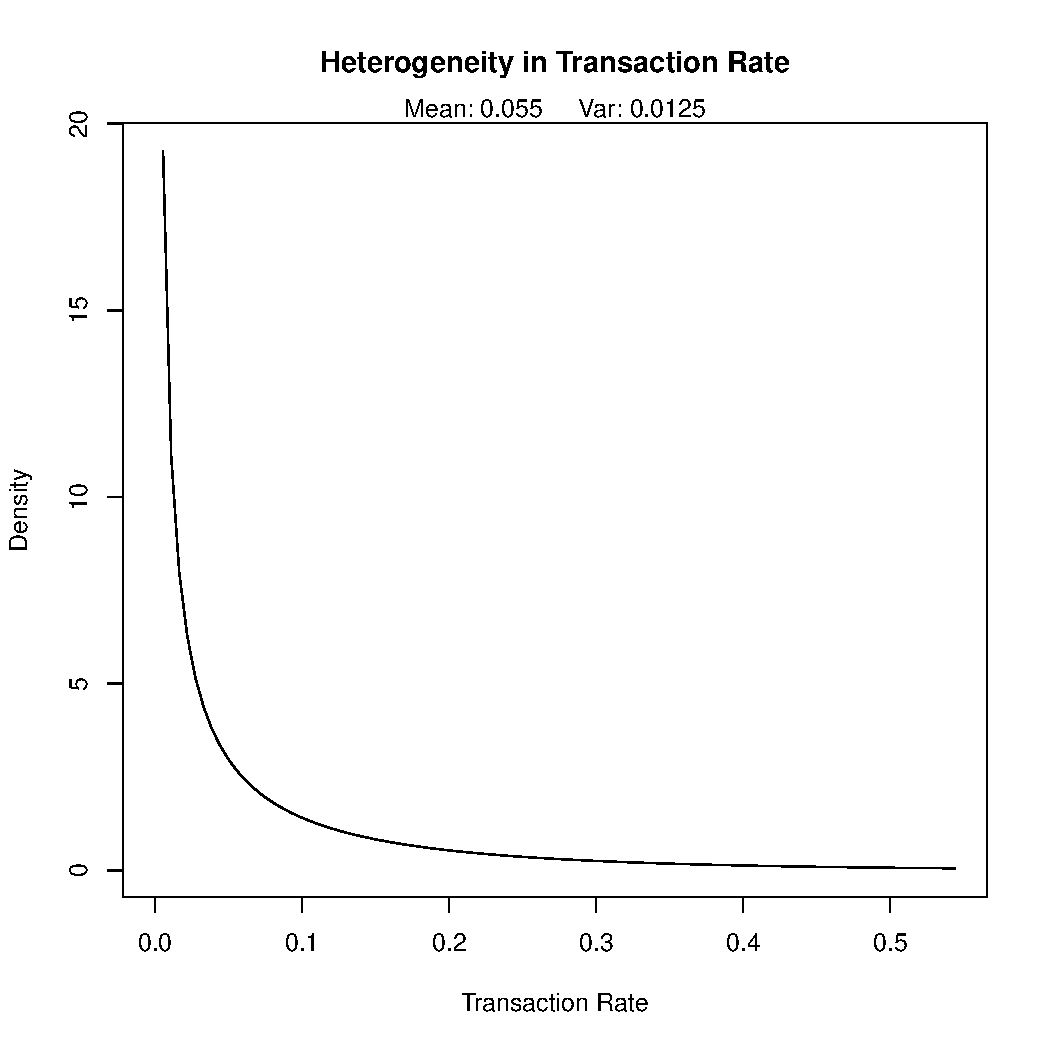
\includegraphics[width=0.6\textwidth]{figure/bgnbdTransactionHeterogeneity}
  \caption{Transaction rate heterogeneity of estimated parameters.}\label{fig:bgnbdTransactionHeterogeneity}
  \end{center}
\end{figure}
      


\begin{figure}
  \begin{center}
  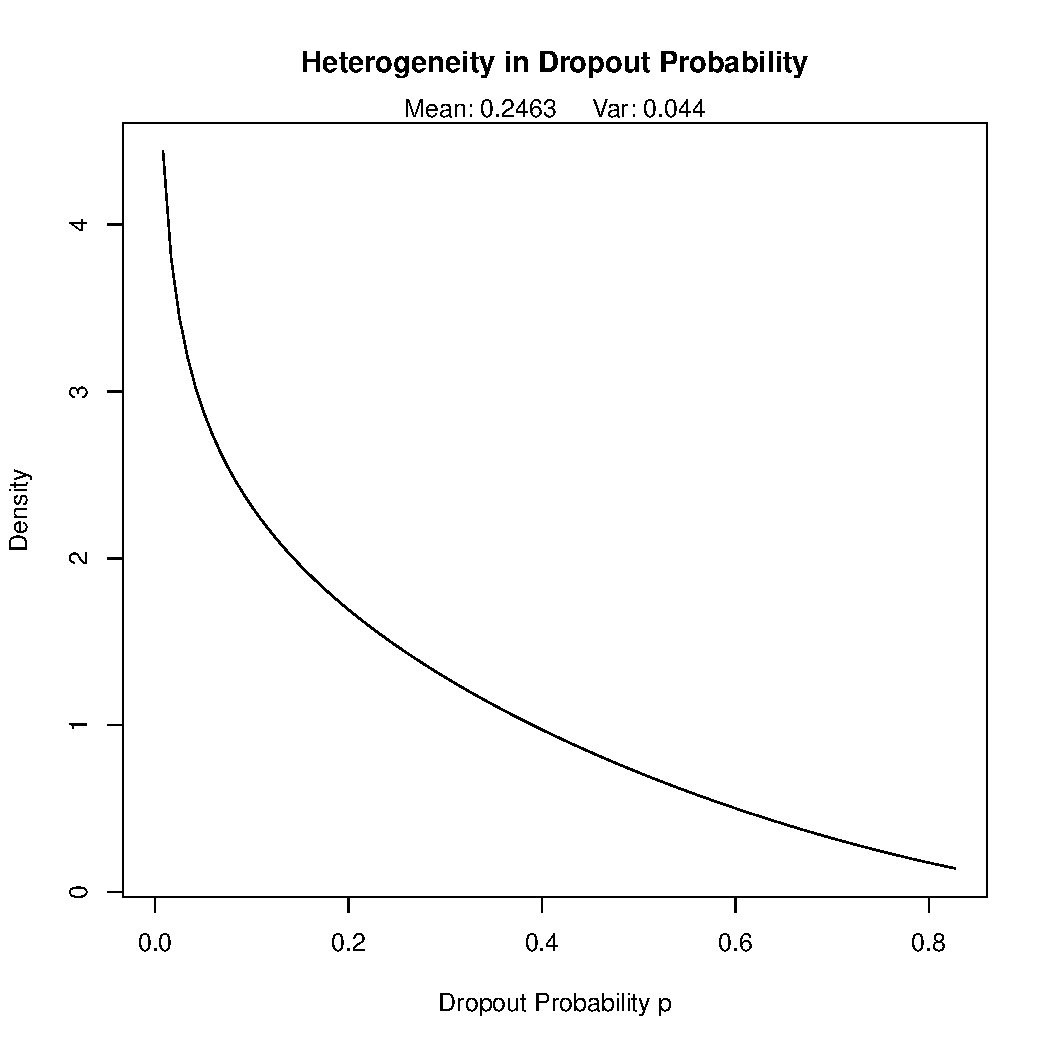
\includegraphics[width=0.6\textwidth]{figure/bgnbdDropoutHeterogeneity}
  \caption{Dropout probability heterogeneity of estimated parameters.}\label{fig:bgnbdDropoutHeterogeneity}
  \end{center}
\end{figure}
 
\subsection{Individual Level Estimations}
Now that we have parameters for the population, we can make
estimations for customers on the individual level.

First, we can estimate the number of transactions we expect a newly
acquired customer to make in a given time period. Let's say, for
example, that we are interested in the number of repeat transactions a
newly acquired customer will make in a time period of one year. Note
that we use 52 weeks to represent one year, not 12 months, 365 days,
or 1 year. This is because our parameters were estimated using weekly
data.

\begin{knitrout}
\definecolor{shadecolor}{rgb}{0.969, 0.969, 0.969}\color{fgcolor}\begin{kframe}
\begin{alltt}
\hlkwd{bgnbd.Expectation}\hlstd{(params,} \hlkwc{t}\hlstd{=}\hlnum{52}\hlstd{);}
\end{alltt}
\begin{verbatim}
#       p3 
# 1.444004
\end{verbatim}
\end{kframe}
\end{knitrout}

We can also obtain expected characteristics for a specific customer,
conditional on their purchasing behavior during the calibration
period. The first of these is
\texttt{bgnbd.ConditionalExpectedTransactions}, which gives the number
of transactions we expect a customer to make in the holdout
period. The second is \texttt{bgnbd.PAlive}, which gives the
probability that a customer is still alive at the end of the
calibration period. As above, the time periods used depend on which
time period was used to estimate the parameters. 

\begin{knitrout}
\definecolor{shadecolor}{rgb}{0.969, 0.969, 0.969}\color{fgcolor}\begin{kframe}
\begin{alltt}
\hlstd{cal.cbs[}\hlstr{"1516"}\hlstd{,]}
\end{alltt}
\begin{verbatim}
#        x      t.x    T.cal 
# 26.00000 30.85714 31.00000
\end{verbatim}
\begin{alltt}
\hlstd{x} \hlkwb{<-} \hlstd{cal.cbs[}\hlstr{"1516"}\hlstd{,} \hlstr{"x"}\hlstd{]}
\hlstd{t.x} \hlkwb{<-} \hlstd{cal.cbs[}\hlstr{"1516"}\hlstd{,} \hlstr{"t.x"}\hlstd{]}
\hlstd{T.cal} \hlkwb{<-} \hlstd{cal.cbs[}\hlstr{"1516"}\hlstd{,} \hlstr{"T.cal"}\hlstd{]}
\hlkwd{bgnbd.ConditionalExpectedTransactions}\hlstd{(params,} \hlkwc{T.star} \hlstd{=} \hlnum{52}\hlstd{,}
                                     \hlstd{x, t.x, T.cal)}
\end{alltt}
\begin{verbatim}
#       p3 
# 25.75659
\end{verbatim}
\begin{alltt}
\hlkwd{bgnbd.PAlive}\hlstd{(params, x, t.x, T.cal)}
\end{alltt}
\begin{verbatim}
#        p3 
# 0.9688523
\end{verbatim}
\end{kframe}
\end{knitrout}

There is one more point to note here---using the conditional
expectation function, we can see the ``increasing frequency paradox''
in action:

\begin{knitrout}
\definecolor{shadecolor}{rgb}{0.969, 0.969, 0.969}\color{fgcolor}\begin{kframe}
\begin{alltt}
\hlkwa{for} \hlstd{(i} \hlkwa{in} \hlkwd{seq}\hlstd{(}\hlnum{10}\hlstd{,} \hlnum{25}\hlstd{,} \hlnum{5}\hlstd{))\{}
  \hlstd{cond.expectation} \hlkwb{<-} \hlkwd{bgnbd.ConditionalExpectedTransactions}\hlstd{(}
                        \hlstd{params,} \hlkwc{T.star} \hlstd{=} \hlnum{52}\hlstd{,} \hlkwc{x} \hlstd{= i,}
                        \hlkwc{t.x} \hlstd{=} \hlnum{20}\hlstd{,} \hlkwc{T.cal} \hlstd{=} \hlnum{39}\hlstd{)}
  \hlkwd{cat} \hlstd{(}\hlstr{"x:"}\hlstd{,i,}\hlstr{"\textbackslash{}t Expectation:"}\hlstd{,cond.expectation,} \hlkwc{fill} \hlstd{=} \hlnum{TRUE}\hlstd{)}
\hlstd{\}}
\end{alltt}
\begin{verbatim}
# x: 10 	 Expectation: 0.3474606
# x: 15 	 Expectation: 0.04283391
# x: 20 	 Expectation: 0.004158973
# x: 25 	 Expectation: 0.0003583685
\end{verbatim}
\end{kframe}
\end{knitrout}

\subsection{Plotting/ Goodness-of-fit}
\label{subsec:bgnbdPlotting}
We would like to be able to do more than make inferences about
individual customers. The BTYD package provides functions to plot
expected customer behavior against actual customer behaviour in the
both the calibration and holdout periods.

The first such function is the obvious starting point: a comparison of
actual and expected frequencies within the calibration period. This is
figure \ref{fig:bgnbdCalibrationFit}, which was generated using the
following code:

\begin{knitrout}
\definecolor{shadecolor}{rgb}{0.969, 0.969, 0.969}\color{fgcolor}\begin{kframe}
\begin{alltt}
\hlkwd{bgnbd.PlotFrequencyInCalibration}\hlstd{(params, cal.cbs,} \hlnum{7}\hlstd{)}
\end{alltt}
\end{kframe}
\end{knitrout}

This function obviously needs to be able to generate expected data
(from estimated parameters) and requires the actual data (the
calibration period customer-by-sufficient-statistic).  It also
requires another number, called the censor number. The histogram that
is plotted is right-censored; after a certain number, all frequencies
are binned together. The number provided as a censor number determines
where the data is cut off.

Unfortunately, the only thing we can tell from comparing calibration
period frequencies is that the fit between our model and the data
isn't awful. We need to verify that the fit of the model holds into
the holdout period. Firstly, however, we are are going to need to get
information for holdout period. \texttt{dc.ElogToCbsCbt} produces both
a calibration period customer-by-sufficient-statistic matrix and a
holdout period customer-by-sufficient-statistic matrix, which could be
combined in order to find the number of transactions each customer
made in the holdout period. However, since we did not use
\texttt{dc.ElogToCbsCbt}, I am going to get the information directly
from the event log. Note that I subtract the number of repeat
transactions in the calibration period from the total number of
transactions. We remove the initial transactions first as we are not
concerned with them.

\begin{knitrout}
\definecolor{shadecolor}{rgb}{0.969, 0.969, 0.969}\color{fgcolor}\begin{kframe}
\begin{alltt}
\hlstd{elog} \hlkwb{<-} \hlkwd{dc.SplitUpElogForRepeatTrans}\hlstd{(elog)}\hlopt{$}\hlstd{repeat.trans.elog;}
\hlstd{x.star} \hlkwb{<-} \hlkwd{rep}\hlstd{(}\hlnum{0}\hlstd{,} \hlkwd{nrow}\hlstd{(cal.cbs));}
\hlstd{cal.cbs} \hlkwb{<-} \hlkwd{cbind}\hlstd{(cal.cbs, x.star);}
\hlstd{elog.custs} \hlkwb{<-} \hlstd{elog}\hlopt{$}\hlstd{cust;}
\hlkwa{for} \hlstd{(i} \hlkwa{in} \hlnum{1}\hlopt{:}\hlkwd{nrow}\hlstd{(cal.cbs))\{}
  \hlstd{current.cust} \hlkwb{<-} \hlkwd{rownames}\hlstd{(cal.cbs)[i]}
  \hlstd{tot.cust.trans} \hlkwb{<-} \hlkwd{length}\hlstd{(}\hlkwd{which}\hlstd{(elog.custs} \hlopt{==} \hlstd{current.cust))}
  \hlstd{cal.trans} \hlkwb{<-} \hlstd{cal.cbs[i,} \hlstr{"x"}\hlstd{]}
  \hlstd{cal.cbs[i,} \hlstr{"x.star"}\hlstd{]} \hlkwb{<-}  \hlstd{tot.cust.trans} \hlopt{-} \hlstd{cal.trans}
\hlstd{\}}
\hlstd{cal.cbs[}\hlnum{1}\hlopt{:}\hlnum{3}\hlstd{,]}
\end{alltt}
\begin{verbatim}
#   x       t.x    T.cal x.star
# 1 2 30.428571 38.85714      1
# 2 1  1.714286 38.85714      0
# 3 0  0.000000 38.85714      0
\end{verbatim}
\end{kframe}
\end{knitrout}

Now we can see how well our model does in the holdout period. Figure
\ref{fig:bgnbdCondExpComp} shows the output produced by the code below. It
divides the customers up into bins according to calibration period
frequencies and plots actual and conditional expected holdout period
frequencies for these bins.

\begin{knitrout}\small
\definecolor{shadecolor}{rgb}{0.969, 0.969, 0.969}\color{fgcolor}\begin{kframe}
\begin{alltt}
\hlstd{T.star} \hlkwb{<-} \hlnum{39} \hlcom{# length of the holdout period}
\hlstd{censor} \hlkwb{<-} \hlnum{7}  \hlcom{# This censor serves the same purpose described above}
\hlstd{x.star} \hlkwb{<-} \hlstd{cal.cbs[,}\hlstr{"x.star"}\hlstd{]}

\hlkwd{pdf}\hlstd{(}\hlkwc{file} \hlstd{=} \hlstr{'figure/bgnbdCondExpComp.pdf'}\hlstd{)}
\hlstd{comp} \hlkwb{<-} \hlkwd{bgnbd.PlotFreqVsConditionalExpectedFrequency}\hlstd{(params, T.star,}
                                              \hlstd{cal.cbs, x.star, censor)}
\hlkwd{dev.off}\hlstd{()}
\end{alltt}
\begin{verbatim}
# pdf 
#   2
\end{verbatim}
\begin{alltt}
\hlkwd{rownames}\hlstd{(comp)} \hlkwb{<-} \hlkwd{c}\hlstd{(}\hlstr{"act"}\hlstd{,} \hlstr{"exp"}\hlstd{,} \hlstr{"bin"}\hlstd{)}
\hlstd{comp}
\end{alltt}
\begin{verbatim}
#           freq.0      freq.1     freq.2     freq.3    freq.4    freq.5
# act    0.2367116   0.6970387   1.392523   1.560000  2.532258  2.947368
# exp    0.2250893   0.5231364   1.044126   1.520256  2.163824  2.653789
# bin 1411.0000000 439.0000000 214.000000 100.000000 62.000000 38.000000
#        freq.6   freq.7+
# act  3.862069  6.359375
# exp  3.503957  6.157036
# bin 29.000000 64.000000
\end{verbatim}
\end{kframe}
\end{knitrout}

\begin{figure}
  \begin{center}
  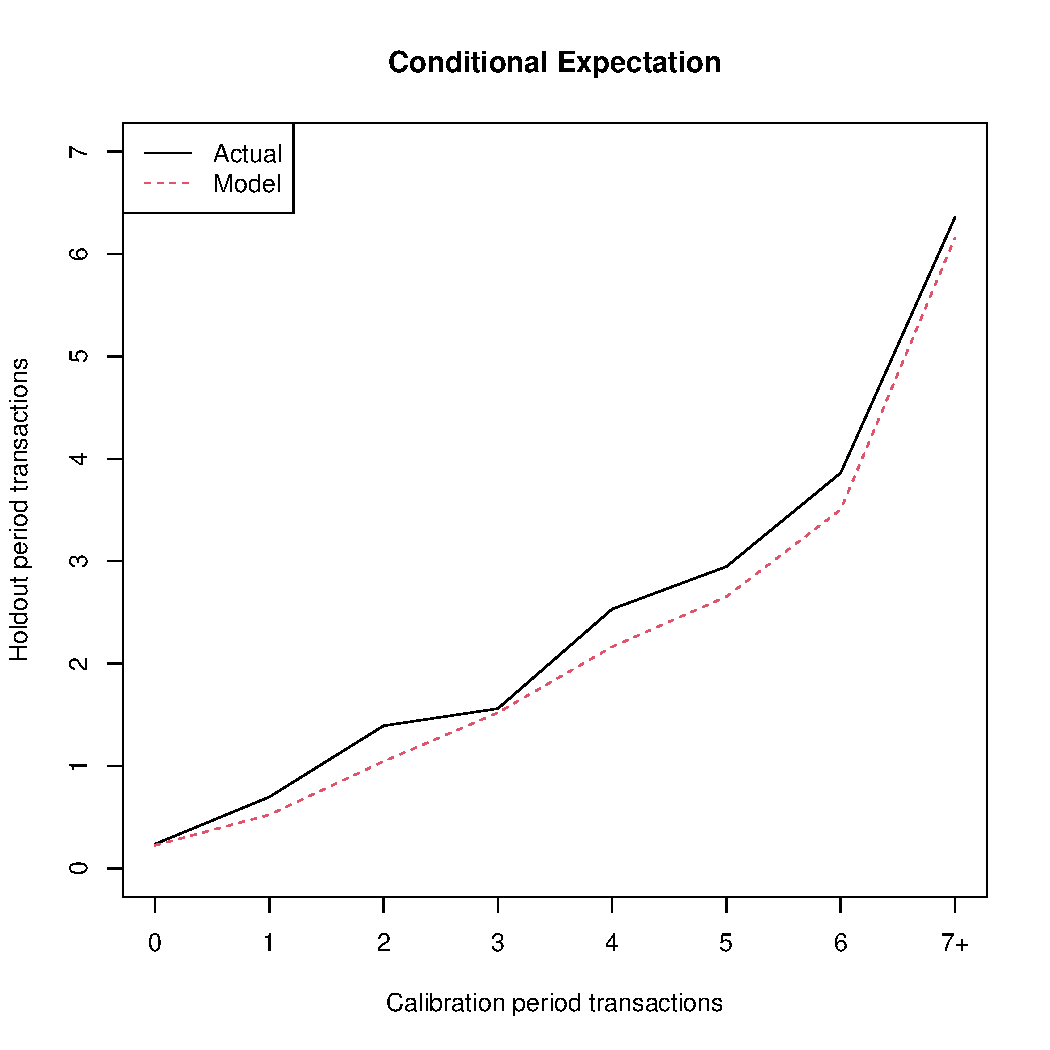
\includegraphics[width=0.6\textwidth]{figure/bgnbdCondExpComp}
  \caption{Actual vs. conditional expected transactions in the holdout period.}\label{fig:bgnbdCondExpComp}
  \end{center}
\end{figure}

As you can see above, the graph also produces a matrix output. Most
plotting functions in the BTYD package produce output like this. They
are often worth looking at because they contain additional information
not presented in the graph---the size of each bin in the graph. In
this graph, for example, this information is important because the bin
sizes show that the gap at zero means a lot more than the precision at
6 or 7 transactions. Despite this, this graph shows that the model
fits the data very well in the holdout period.

Aggregation by calibration period frequency is just one way to do
it. BTYD also provides plotting functions which aggregate by several
other measures. The other one I will demonstrate here is aggregation
by time---how well does our model predict how many transactions will
occur in each week?

The first step, once again, is going to be to collect the data we need
to compare the model to. The customer-by-time matrix has already
collected the data for us by time period; so we'll use that to gather
the total transactions per day. Then we convert the daily tracking
data to weekly data.

\begin{knitrout}
\definecolor{shadecolor}{rgb}{0.969, 0.969, 0.969}\color{fgcolor}\begin{kframe}
\begin{alltt}
\hlstd{tot.cbt} \hlkwb{<-} \hlkwd{dc.CreateFreqCBT}\hlstd{(elog)}
\end{alltt}


{\ttfamily\noindent\itshape\color{messagecolor}{\# ...Completed Freq CBT}}\begin{alltt}
\hlstd{d.track.data} \hlkwb{<-} \hlkwd{rep}\hlstd{(}\hlnum{0}\hlstd{,} \hlnum{7} \hlopt{*} \hlnum{78}\hlstd{)}
\hlstd{origin} \hlkwb{<-} \hlkwd{as.Date}\hlstd{(}\hlstr{"1997-01-01"}\hlstd{)}
\hlkwa{for} \hlstd{(i} \hlkwa{in} \hlkwd{colnames}\hlstd{(tot.cbt))\{}
  \hlstd{date.index} \hlkwb{<-} \hlkwd{difftime}\hlstd{(}\hlkwd{as.Date}\hlstd{(i), origin)} \hlopt{+} \hlnum{1}\hlstd{;}
  \hlstd{d.track.data[date.index]} \hlkwb{<-} \hlkwd{sum}\hlstd{(tot.cbt[,i]);}
\hlstd{\}}
\hlstd{w.track.data} \hlkwb{<-}  \hlkwd{rep}\hlstd{(}\hlnum{0}\hlstd{,} \hlnum{78}\hlstd{)}
\hlkwa{for} \hlstd{(j} \hlkwa{in} \hlnum{1}\hlopt{:}\hlnum{78}\hlstd{)\{}
  \hlstd{w.track.data[j]} \hlkwb{<-} \hlkwd{sum}\hlstd{(d.track.data[(j}\hlopt{*}\hlnum{7}\hlopt{-}\hlnum{6}\hlstd{)}\hlopt{:}\hlstd{(j}\hlopt{*}\hlnum{7}\hlstd{)])}
\hlstd{\}}
\end{alltt}
\end{kframe}
\end{knitrout}

Now, we can make a plot comparing the actual number of transactions to
the expected number of transactions on a weekly basis, as shown in
figure \ref{fig:bgnbdTrackingInc}. Note that we set
\texttt{n.periods.final} to 78. This is to show that we are working
with weekly data. If our tracking data was daily, we would use 546
here---the function would plot our daily tracking data against
expected daily transactions, instead of plotting our weekly tracking
data against expected weekly transactions. This concept may be a bit
tricky, but is explained in the documentation for
\texttt{bgnbd.PlotTrackingInc}. The reason there are two numbers for
the total period (\texttt{T.tot} and \texttt{n.periods.final}) is that
your customer-by-sufficient-statistic matrix and your tracking data
may be in different time periods.

\begin{knitrout}
\definecolor{shadecolor}{rgb}{0.969, 0.969, 0.969}\color{fgcolor}\begin{kframe}
\begin{alltt}
\hlstd{T.cal} \hlkwb{<-} \hlstd{cal.cbs[,}\hlstr{"T.cal"}\hlstd{]}
\hlstd{T.tot} \hlkwb{<-} \hlnum{78}
\hlstd{n.periods.final} \hlkwb{<-} \hlnum{78}
\hlkwd{pdf}\hlstd{(}\hlkwc{file} \hlstd{=} \hlstr{'figure/bgnbdTrackingInc.pdf'}\hlstd{)}
\hlstd{inc.tracking} \hlkwb{<-} \hlkwd{bgnbd.PlotTrackingInc}\hlstd{(params,}
                                      \hlstd{T.cal,}
                                      \hlstd{T.tot,}
                                      \hlstd{w.track.data,}
                                      \hlstd{n.periods.final,}
                                      \hlstd{allHardie)}
\hlkwd{dev.off}\hlstd{()}
\end{alltt}
\begin{verbatim}
# pdf 
#   2
\end{verbatim}
\begin{alltt}
\hlstd{inc.tracking[,}\hlnum{20}\hlopt{:}\hlnum{25}\hlstd{]}
\end{alltt}
\begin{verbatim}
#              [,1]     [,2]     [,3]     [,4]     [,5]     [,6]
# actual   73.00000 55.00000 70.00000 33.00000 56.00000 99.00000
# expected 76.86531 74.88843 73.04554 71.32166 69.70412 68.18213
\end{verbatim}
\end{kframe}
\end{knitrout}

\begin{figure}
  \begin{center}
  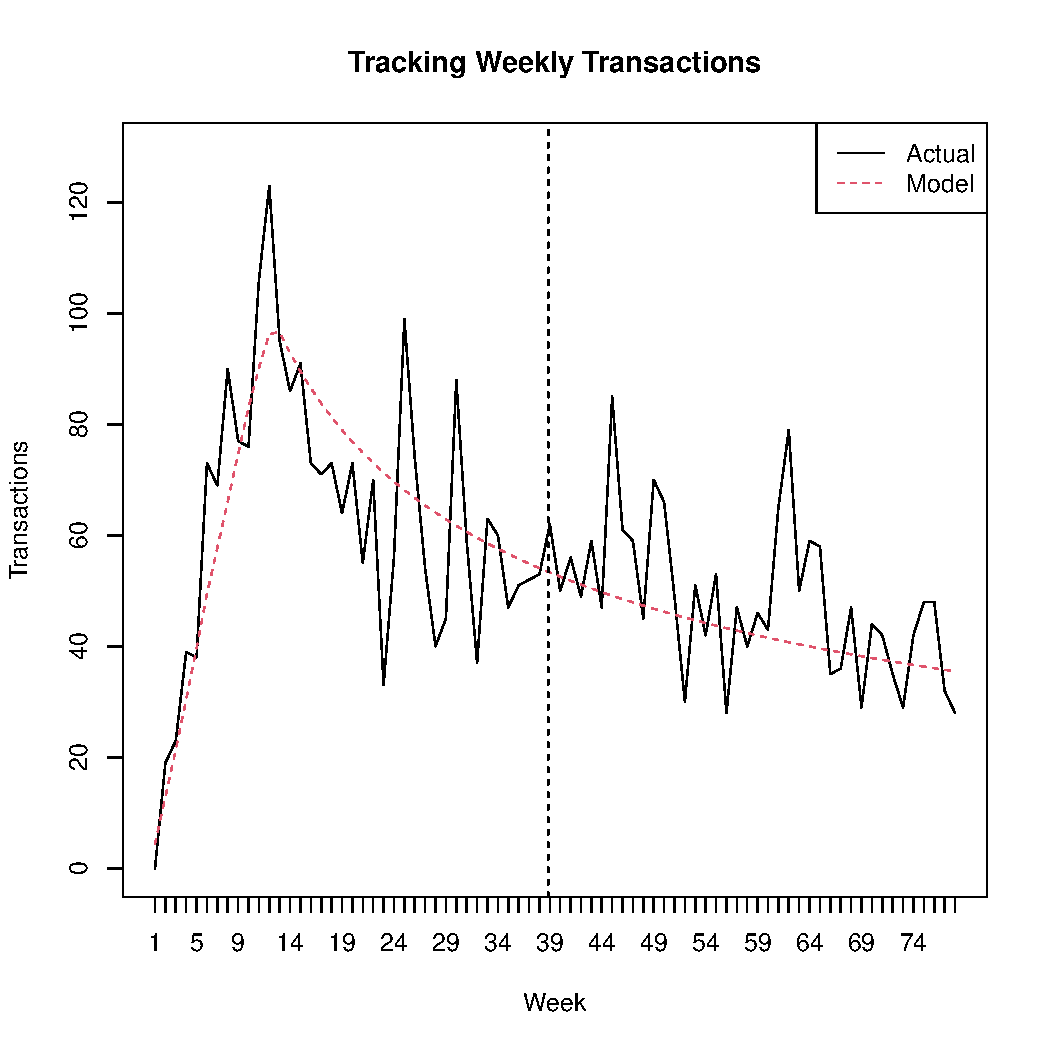
\includegraphics[width=0.6\textwidth]{figure/bgnbdTrackingInc}
  \caption{Actual vs. expected incremental purchasing behaviour.}\label{fig:bgnbdTrackingInc}
  \end{center}
\end{figure}

Although figure \ref{fig:bgnbdTrackingInc} shows that the model is
definitely capturing the trend of customer purchases over time, it is
very messy and may not convince skeptics. Furthermore, the matrix, of
which a sample is shown, does not really convey much information since
purchases can vary so much from one week to the next. For these
reasons, we may need to smooth the data out by cumulating it over
time, as shown in Figure \ref{fig:bgnbdTrackingCum}.

\begin{knitrout}
\definecolor{shadecolor}{rgb}{0.969, 0.969, 0.969}\color{fgcolor}\begin{kframe}
\begin{alltt}
\hlstd{cum.tracking.data} \hlkwb{<-} \hlkwd{cumsum}\hlstd{(w.track.data)}
\hlkwd{pdf}\hlstd{(}\hlkwc{file} \hlstd{=} \hlstr{'figure/bgnbdTrackingCum.pdf'}\hlstd{)}
\hlstd{cum.tracking} \hlkwb{<-} \hlkwd{bgnbd.PlotTrackingCum}\hlstd{(params,}
                                      \hlstd{T.cal,}
                                      \hlstd{T.tot,}
                                      \hlstd{cum.tracking.data,}
                                      \hlstd{n.periods.final,}
                                      \hlstd{allHardie)}
\hlkwd{dev.off}\hlstd{()}
\end{alltt}
\begin{verbatim}
# pdf 
#   2
\end{verbatim}
\begin{alltt}
\hlstd{cum.tracking[,}\hlnum{20}\hlopt{:}\hlnum{25}\hlstd{]}
\end{alltt}
\begin{verbatim}
#              [,1]     [,2]     [,3]     [,4]     [,5]   [,6]
# actual   1359.000 1414.000 1484.000 1517.000 1573.000 1672.0
# expected 1312.458 1387.346 1460.392 1531.713 1601.418 1669.6
\end{verbatim}
\end{kframe}
\end{knitrout}

\begin{figure}
  \begin{center}
  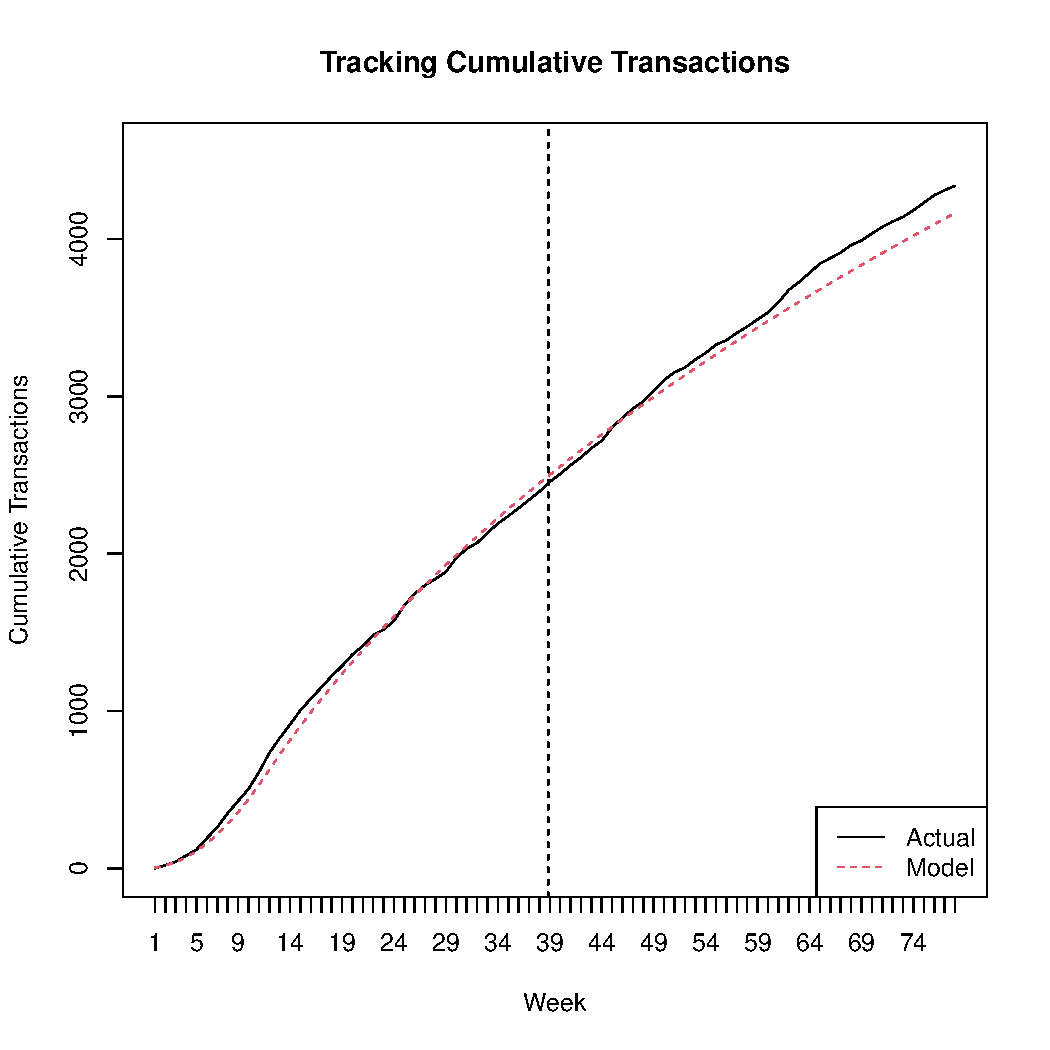
\includegraphics[width=0.6\textwidth]{figure/bgnbdTrackingCum}
  \caption{Actual vs. expected cumulative purchasing behaviour.}\label{fig:bgnbdTrackingCum}
  \end{center}
\end{figure}







\section{BG/BB}

The BG/BB model is also used for non-contractual settings. In many
regards, it is very similar to the Pareto/NBD model---it also uses
four parameters to describe a purchasing process and a dropout
process. The difference between the models is that the BG/BB is used
to describe situations in which customers have discrete transaction
opportunities, rather than being able to make transactions at any
time. For this section, we will be using donation data presented in
Fader et. al. (2010). Figure \ref{fig:bgbbCalibrationFit} shows that
this model also fits the right type of data well.



\begin{figure}
  \begin{center}
  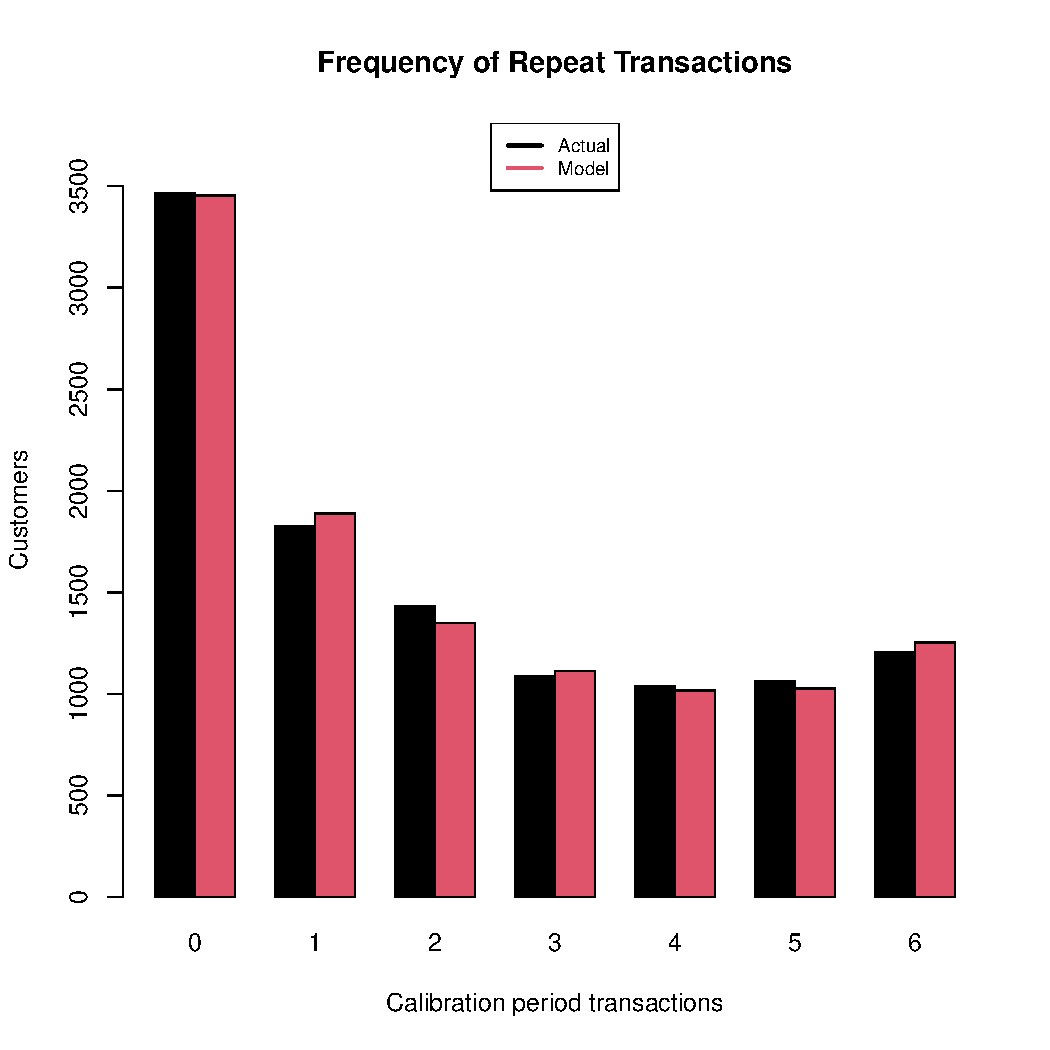
\includegraphics[width=0.6\textwidth]{figure/bgbbCalibrationFit}
  \caption{Calibration period fit of BG/BB model to the donations dataset.}\label{fig:bgbbCalibrationFit}
  \end{center}
\end{figure}

\subsection{Data Preparation}

Luckily, preparing data to be used by the BTYD package BG/BB functions
is going to be very easy if you understood how to set up the data for
the Pareto/NBD package. The BG/BB model uses exactly the same data as
the Pareto/NBD model, but since it is discrete we can go one step
further and create a recency-frequency matrix from our
customer-by-sufficient-statistic matrix. We are able to do this
because the data is discrete---a recency-frequency matrix consists of
a row for every possible calibration period recency/frequency
combination, and contains the total number of customers which had that
particular combination of recency and frequency. While this is not
strictly necessary, it greatly reduces the amount of space required to
store the data and makes parameter estimation much faster---for the
donation data, for example, there is a reduction from 11,104 rows
(number of customers) down to 22.

Since I don't have access to the original event log for the donation
data, I am going to demonstrate the data preparation process with
simulated data (included in the package):

\begin{knitrout}
\definecolor{shadecolor}{rgb}{0.969, 0.969, 0.969}\color{fgcolor}\begin{kframe}
\begin{alltt}
\hlstd{simElog} \hlkwb{<-} \hlkwd{system.file}\hlstd{(}\hlstr{"data/discreteSimElog.csv"}\hlstd{,}
                       \hlkwc{package} \hlstd{=} \hlstr{"BTYD"}\hlstd{)}
\hlstd{elog} \hlkwb{<-} \hlkwd{dc.ReadLines}\hlstd{(simElog,} \hlkwc{cust.idx} \hlstd{=} \hlnum{1}\hlstd{,} \hlkwc{date.idx} \hlstd{=} \hlnum{2}\hlstd{)}
\hlstd{elog[}\hlnum{1}\hlopt{:}\hlnum{3}\hlstd{,]}
\end{alltt}
\begin{verbatim}
#   cust       date
# 1    1 1970-01-01
# 2    1 1975-01-01
# 3    1 1977-01-01
\end{verbatim}
\begin{alltt}
\hlstd{elog}\hlopt{$}\hlstd{date} \hlkwb{<-} \hlkwd{as.Date}\hlstd{(elog}\hlopt{$}\hlstd{date,} \hlstr{"%Y-%m-%d"}\hlstd{)}

\hlkwd{max}\hlstd{(elog}\hlopt{$}\hlstd{date);}
\end{alltt}
\begin{verbatim}
# [1] "1983-01-01"
\end{verbatim}
\begin{alltt}
\hlkwd{min}\hlstd{(elog}\hlopt{$}\hlstd{date);}
\end{alltt}
\begin{verbatim}
# [1] "1970-01-01"
\end{verbatim}
\begin{alltt}
\hlcom{# let's make the calibration period end somewhere in-between}
\hlstd{T.cal} \hlkwb{<-} \hlkwd{as.Date}\hlstd{(}\hlstr{"1977-01-01"}\hlstd{)}

\hlstd{simData} \hlkwb{<-} \hlkwd{dc.ElogToCbsCbt}\hlstd{(elog,} \hlkwc{per}\hlstd{=}\hlstr{"year"}\hlstd{, T.cal)}
\hlstd{cal.cbs} \hlkwb{<-} \hlstd{simData}\hlopt{$}\hlstd{cal}\hlopt{$}\hlstd{cbs}

\hlstd{freq}\hlkwb{<-} \hlstd{cal.cbs[,}\hlstr{"x"}\hlstd{]}
\hlstd{rec} \hlkwb{<-} \hlstd{cal.cbs[,}\hlstr{"t.x"}\hlstd{]}
\hlstd{trans.opp} \hlkwb{<-} \hlnum{7} \hlcom{# transaction opportunities}
\hlstd{cal.rf.matrix} \hlkwb{<-} \hlkwd{dc.MakeRFmatrixCal}\hlstd{(freq, rec, trans.opp)}
\hlstd{cal.rf.matrix[}\hlnum{1}\hlopt{:}\hlnum{5}\hlstd{,]}
\end{alltt}
\begin{verbatim}
#      x t.x n.cal custs
# [1,] 0   0     7  2900
# [2,] 1   1     7   933
# [3,] 1   2     7   218
# [4,] 2   2     7   489
# [5,] 1   3     7    95
\end{verbatim}
\end{kframe}
\end{knitrout}

\subsection{Parameter Estimation}

Estimating BG/BB parameters is very similar to estimating Pareto/NBD
parameters. The same rules apply---we use
\texttt{bgbb.EstimateParameters}, which also uses (1,1,1,1) as default
starting parameters. Once again, we should run the estimation several
times with its own output as starting parameters, to make sure that
our estimation converges. One should also test the estimation from
different starting points, but I am not going to do that here.

\begin{knitrout}
\definecolor{shadecolor}{rgb}{0.969, 0.969, 0.969}\color{fgcolor}\begin{kframe}
\begin{alltt}
\hlkwd{data}\hlstd{(donationsSummary);}
\hlstd{rf.matrix} \hlkwb{<-} \hlstd{donationsSummary}\hlopt{$}\hlstd{rf.matrix}
\hlstd{params} \hlkwb{<-} \hlkwd{bgbb.EstimateParameters}\hlstd{(rf.matrix);}
\hlstd{LL} \hlkwb{<-} \hlkwd{bgbb.rf.matrix.LL}\hlstd{(params, rf.matrix);}
\hlstd{p.matrix} \hlkwb{<-} \hlkwd{c}\hlstd{(params, LL);}
\hlkwa{for} \hlstd{(i} \hlkwa{in} \hlnum{1}\hlopt{:}\hlnum{2}\hlstd{)\{}
\hlstd{params} \hlkwb{<-} \hlkwd{bgbb.EstimateParameters}\hlstd{(rf.matrix, params);}
\hlstd{LL} \hlkwb{<-} \hlkwd{bgbb.rf.matrix.LL}\hlstd{(params, rf.matrix);}
\hlstd{p.matrix.row} \hlkwb{<-} \hlkwd{c}\hlstd{(params, LL);}
\hlstd{p.matrix} \hlkwb{<-} \hlkwd{rbind}\hlstd{(p.matrix, p.matrix.row);}
\hlstd{\}}
\hlkwd{colnames}\hlstd{(p.matrix)} \hlkwb{<-} \hlkwd{c}\hlstd{(}\hlstr{"alpha"}\hlstd{,} \hlstr{"beta"}\hlstd{,} \hlstr{"gamma"}\hlstd{,} \hlstr{"delta"}\hlstd{,} \hlstr{"LL"}\hlstd{);}
\hlkwd{rownames}\hlstd{(p.matrix)} \hlkwb{<-} \hlnum{1}\hlopt{:}\hlnum{3}\hlstd{;}
\hlstd{p.matrix;}
\end{alltt}
\begin{verbatim}
#      alpha      beta     gamma    delta        LL
# 1 1.203507 0.7497667 0.6567568 2.783887 -33225.58
# 2 1.203533 0.7497272 0.6567788 2.783812 -33225.58
# 3 1.203528 0.7497260 0.6567808 2.783796 -33225.58
\end{verbatim}
\end{kframe}
\end{knitrout}

The parameter estimation converges very quickly. It is much easier,
and faster, to estimate BG/BB parameters than it is to estimate
Pareto/NBD parameters, because there are fewer calculations involved.

We can interpret these parameters by plotting the mixing
distributions. Alpha and beta describe the beta mixing distribution of
the beta-Bernoulli transaction process. We can see the beta
distribution with parameters alpha and beta in figure
\ref{fig:bgbbTransactionHeterogeneity}, plotted using
\texttt{bgbb.PlotTransactionRateHeterogeneity(params)}. Gamma and
Delta describe the beta mixing distribution of the beta-geometric
dropout process. We can see the beta distribution with parameters
gamma and delta in figure \ref{fig:bgbbDropoutHeterogeneity}, plotted
using \texttt{bgbb.PlotDropoutHeterogeneity(params)}. The story told
by these plots describes the type of customers most firms would
want---their transaction parameters are more likely to be high, and
their dropout parameters are more likely to be low.



\begin{figure}
  \begin{center}
  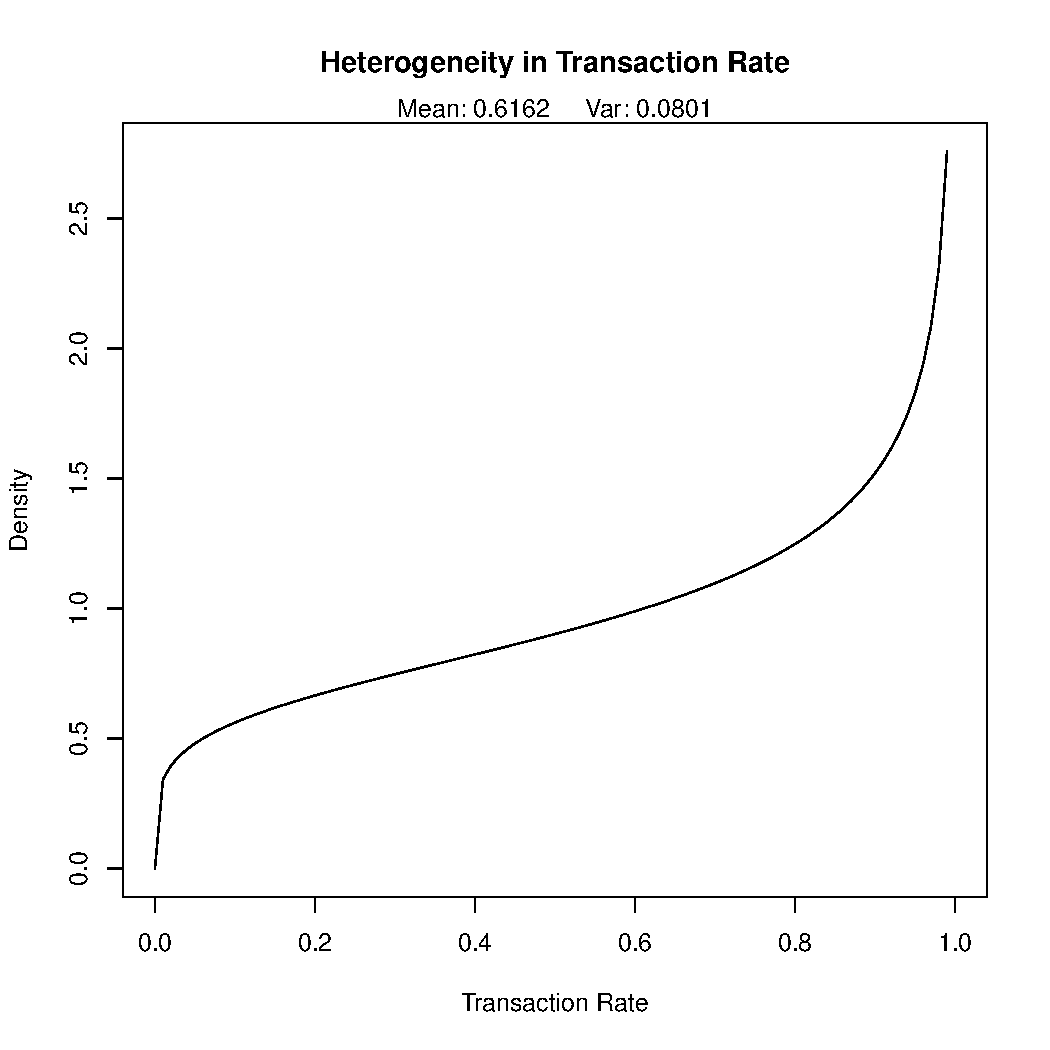
\includegraphics[width=0.6\textwidth]{figure/bgbbTransactionHeterogeneity}
  \caption{Transaction rate heterogeneity of estimated parameters.}\label{fig:bgbbTransactionHeterogeneity}
  \end{center}
\end{figure}
      


\begin{figure}
  \begin{center}
  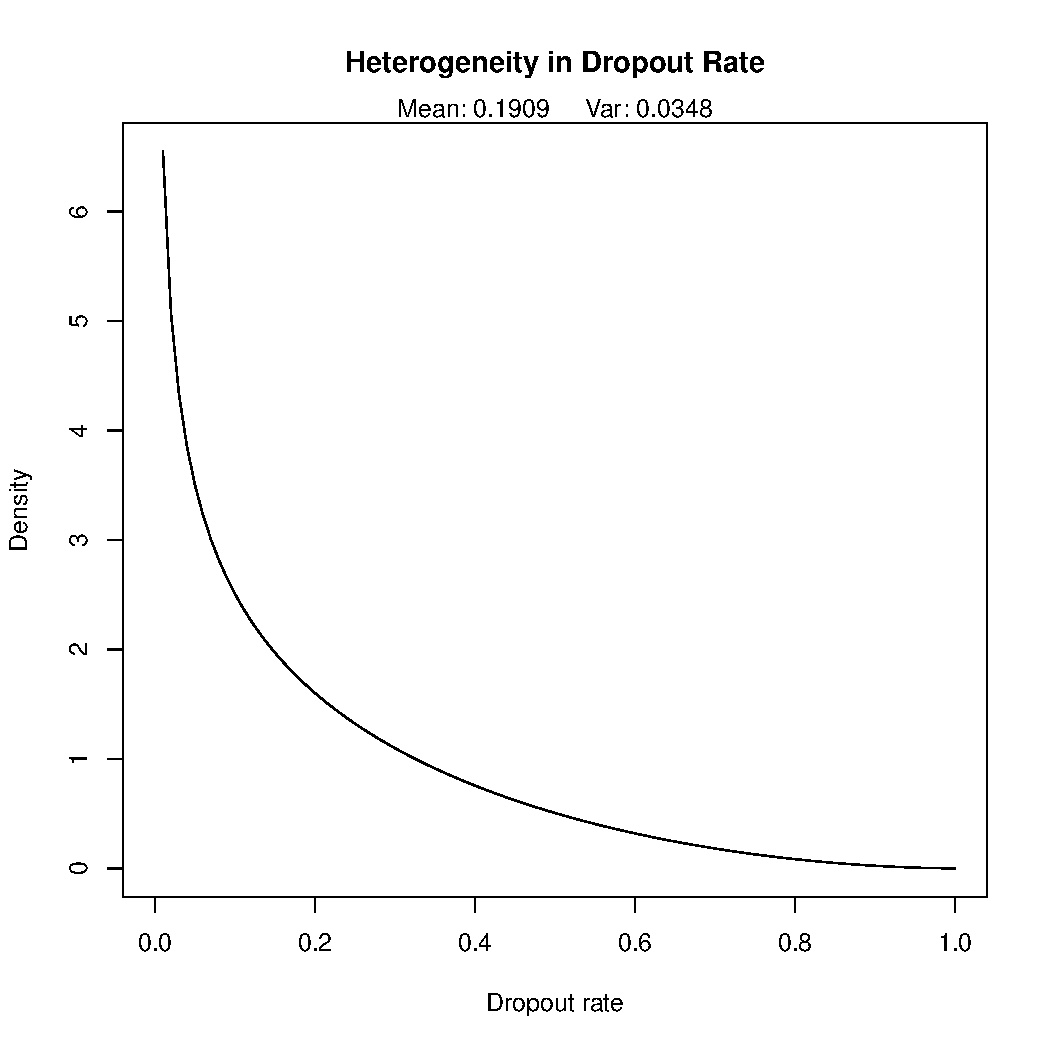
\includegraphics[width=0.6\textwidth]{figure/bgbbDropoutHeterogeneity}
  \caption{Dropout rate heterogeneity of estimated parameters.}\label{fig:bgbbDropoutHeterogeneity}
  \end{center}
\end{figure}

\subsection{Individual Level Estimations}

We can estimate the number of transactions we expect a newly acquired
customer to make in a given time period, just as with the Pareto/NBD
model. For this example, let's say we are interested in estimating the
number of repeat transactions we expect a newly-acquired customer to
make in a period of 10 years. The same rules that we used for
Pareto/NBD functions also apply to BG/BB functions: since we used
years to estimate the parameters, we stick to years to represent time
periods.
\begin{knitrout}
\definecolor{shadecolor}{rgb}{0.969, 0.969, 0.969}\color{fgcolor}\begin{kframe}
\begin{alltt}
\hlkwd{bgbb.Expectation}\hlstd{(params,} \hlkwc{n}\hlstd{=}\hlnum{10}\hlstd{);}
\end{alltt}
\begin{verbatim}
# [1] 3.179805
\end{verbatim}
\end{kframe}
\end{knitrout}


But we want to be able to say something about our existing customers,
not just about a hypothetical customer to be acquired in the
future. Once again, we use conditional expectations for a holdout
period of 10 years. I am going to do this for 2 customers: A, who made
0 transactions in the calibration period; and B, who made 4
transactions in the calibration period, with the last transaction
occuring in the 5th year.

\begin{knitrout}
\definecolor{shadecolor}{rgb}{0.969, 0.969, 0.969}\color{fgcolor}\begin{kframe}
\begin{alltt}
\hlcom{# customer A}
\hlstd{n.cal} \hlkwb{=} \hlnum{6}
\hlstd{n.star} \hlkwb{=} \hlnum{10}
\hlstd{x} \hlkwb{=} \hlnum{0}
\hlstd{t.x} \hlkwb{=} \hlnum{0}
\hlkwd{bgbb.ConditionalExpectedTransactions}\hlstd{(params, n.cal,}
                                     \hlstd{n.star, x, t.x)}
\end{alltt}
\begin{verbatim}
# [1] 0.1302169
\end{verbatim}
\begin{alltt}
\hlcom{# customer B}
\hlstd{x} \hlkwb{=} \hlnum{4}
\hlstd{t.x} \hlkwb{=} \hlnum{5}
\hlkwd{bgbb.ConditionalExpectedTransactions}\hlstd{(params, n.cal,}
                                     \hlstd{n.star, x, t.x)}
\end{alltt}
\begin{verbatim}
# [1] 3.627858
\end{verbatim}
\end{kframe}
\end{knitrout}

As expected, B's conditional expectation is much higher than A's. The
point I am trying to make, however, is that there are 3464 A's in this
dataset and only 284 B's---you should never ignore the zeroes in these
models.

\subsection{Plotting/ Goodness-of-fit}

Figure \ref{fig:pnbdCalibrationFit}, is the first plot to test the
goodness-of-fit: a simple calibration period histogram. 

\begin{knitrout}
\definecolor{shadecolor}{rgb}{0.969, 0.969, 0.969}\color{fgcolor}\begin{kframe}
\begin{alltt}
\hlkwd{bgbb.PlotFrequencyInCalibration}\hlstd{(params, rf.matrix)}
\end{alltt}
\end{kframe}
\end{knitrout}

As with the equivalent Pareto/NBD plot, keep in mind that this plot is
only useful for an initial verification that the fit of the BG/BB
model is not terrible.

The next step is to see how well the model performs in the holdout
period. When we used \texttt{dc.ElogToCbsCbt} earlier, we ignored a
lot of the data it generated. It is easy to get the holdout period
frequencies from that data:

\begin{knitrout}
\definecolor{shadecolor}{rgb}{0.969, 0.969, 0.969}\color{fgcolor}\begin{kframe}
\begin{alltt}
\hlstd{holdout.cbs} \hlkwb{<-} \hlstd{simData}\hlopt{$}\hlstd{holdout}\hlopt{$}\hlstd{cbs}
\hlstd{x.star} \hlkwb{<-} \hlstd{holdout.cbs[,}\hlstr{"x.star"}\hlstd{]}
\end{alltt}
\end{kframe}
\end{knitrout}
  
At this point, we can switch from simulated data to the real
discrete data (donation data) provided with the package. The holdout
period frequencies for the donations data is included in the
package. Using this information, we can generate figure
\ref{fig:bgbbCondExpComp}, which compares actual and conditional
expected transactions in the holdout period. It bins customers
according to calibration period frequencies.
 
\clearpage

\begin{knitrout}\small
\definecolor{shadecolor}{rgb}{0.969, 0.969, 0.969}\color{fgcolor}\begin{kframe}
\begin{alltt}
\hlstd{n.star} \hlkwb{<-} \hlnum{5} \hlcom{# length of the holdout period}
\hlstd{x.star} \hlkwb{<-} \hlstd{donationsSummary}\hlopt{$}\hlstd{x.star}
\hlkwd{pdf}\hlstd{(}\hlkwc{file} \hlstd{=} \hlstr{'figure/bgbbCondExpComp.pdf'}\hlstd{)}
\hlstd{comp} \hlkwb{<-} \hlkwd{bgbb.PlotFreqVsConditionalExpectedFrequency}\hlstd{(params, n.star,}
                                                    \hlstd{rf.matrix, x.star)}
\hlkwd{dev.off}\hlstd{()}
\end{alltt}
\begin{verbatim}
# pdf 
#   2
\end{verbatim}
\begin{alltt}
\hlkwd{rownames}\hlstd{(comp)} \hlkwb{<-} \hlkwd{c}\hlstd{(}\hlstr{"act"}\hlstd{,} \hlstr{"exp"}\hlstd{,} \hlstr{"bin"}\hlstd{)}
\hlstd{comp}
\end{alltt}
\begin{verbatim}
#           freq.0       freq.1       freq.2      freq.3      freq.4      freq.5
# act 1.743649e-01    0.4328031    0.8125874    1.389862    2.061776    2.642521
# exp 7.286318e-02    0.3248841    0.7089417    1.333666    2.031203    2.784482
# bin 3.464000e+03 1823.0000000 1430.0000000 1085.000000 1036.000000 1063.000000
#          freq.6
# act    3.534497
# exp    3.752500
# bin 1203.000000
\end{verbatim}
\end{kframe}
\end{knitrout}

\begin{figure}
  \begin{center}
  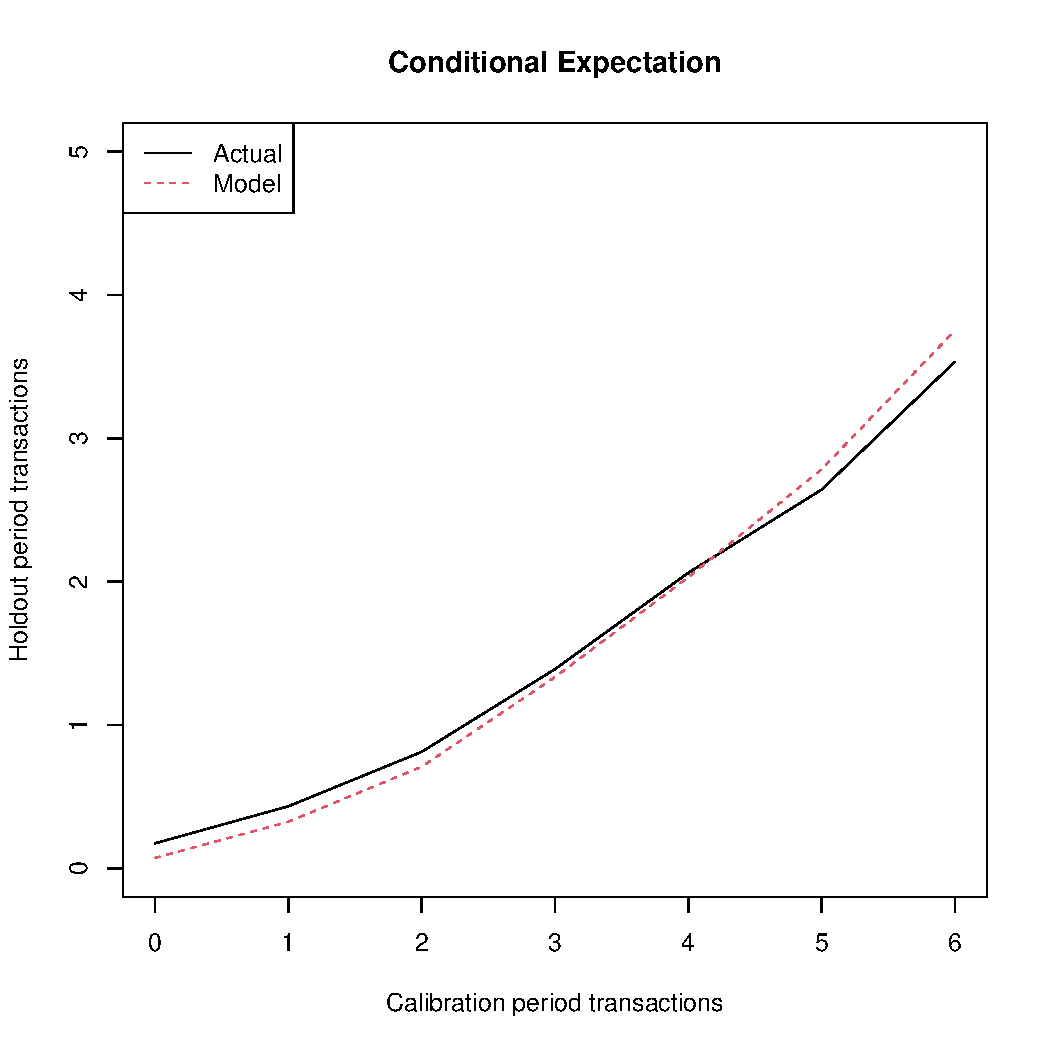
\includegraphics[width=0.6\textwidth]{figure/bgbbCondExpComp}
  \caption{Actual vs. conditional expected transactions in the holdout period, binned by calibration period frequency.}\label{fig:bgbbCondExpComp}
  \end{center}
\end{figure}

Since the BG/BB model uses discrete data, we can also bin customers by
recency. Figure \ref{fig:bgbbCondExpCompRec} shows the fit of holdout
period frequencies, with customers binned in this manner.

\begin{knitrout}\small
\definecolor{shadecolor}{rgb}{0.969, 0.969, 0.969}\color{fgcolor}\begin{kframe}
\begin{alltt}
\hlkwd{pdf}\hlstd{(}\hlkwc{file} \hlstd{=} \hlstr{'figure/bgbbCondExpCompRec.pdf'}\hlstd{)}
\hlstd{comp} \hlkwb{<-} \hlkwd{bgbb.PlotRecVsConditionalExpectedFrequency}\hlstd{(params, n.star,}
                                                   \hlstd{rf.matrix, x.star)}
\hlkwd{dev.off}\hlstd{()}
\end{alltt}
\begin{verbatim}
# pdf 
#   2
\end{verbatim}
\begin{alltt}
\hlkwd{rownames}\hlstd{(comp)} \hlkwb{<-} \hlkwd{c}\hlstd{(}\hlstr{"act"}\hlstd{,} \hlstr{"exp"}\hlstd{,} \hlstr{"bin"}\hlstd{)}
\hlstd{comp}
\end{alltt}
\begin{verbatim}
#            rec.0        rec.1       rec.2       rec.3       rec.4       rec.5
# act 1.743649e-01    0.2181485   0.3898876   0.4872521   0.8088685    1.652289
# exp 7.286318e-02    0.0856939   0.1798423   0.4041111   0.8510811    1.726323
# bin 3.464000e+03 1091.0000000 890.0000000 706.0000000 654.0000000 1136.000000
#           rec.6
# act    2.946886
# exp    3.027190
# bin 3163.000000
\end{verbatim}
\end{kframe}
\end{knitrout}

\begin{figure}
  \begin{center}
  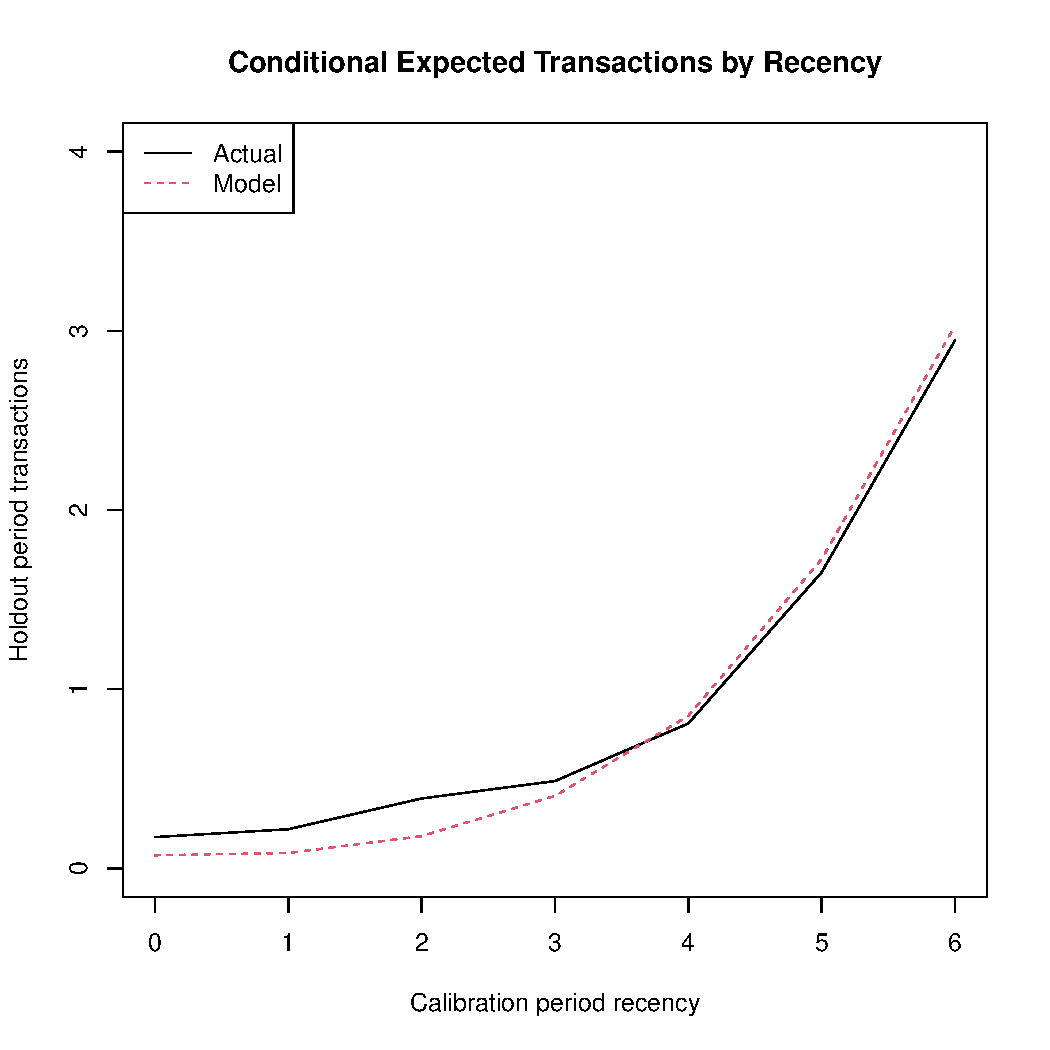
\includegraphics[width=0.6\textwidth]{figure/bgbbCondExpCompRec}
  \caption{Actual vs. conditional expected transactions in the holdout period, binned by calibration period recency.}\label{fig:bgbbCondExpCompRec}
  \end{center}
\end{figure}

Another plotting function provided by the BTYD package is the tracking
function---binning the data according to which time period
transactions occurred in. Since we do not have the granular data
available, we once again cannot get the required data from the event
log; however, the process will be exactly the same as described in
section \ref{subsec:pnbdPlotting}. The annual transaction data is
provided by the package. 

\begin{knitrout}
\definecolor{shadecolor}{rgb}{0.969, 0.969, 0.969}\color{fgcolor}\begin{kframe}
\begin{alltt}
\hlstd{inc.track.data} \hlkwb{<-} \hlstd{donationsSummary}\hlopt{$}\hlstd{annual.trans}
\hlstd{n.cal} \hlkwb{<-} \hlnum{6}
\hlstd{xtickmarks} \hlkwb{<-} \hlnum{1996}\hlopt{:}\hlnum{2006}
\hlkwd{pdf}\hlstd{(}\hlkwc{file} \hlstd{=} \hlstr{'figure/bgbbTrackingInc.pdf'}\hlstd{)}
\hlstd{inc.tracking} \hlkwb{<-} \hlkwd{bgbb.PlotTrackingInc}\hlstd{(params, rf.matrix,}
                                     \hlstd{inc.track.data,}
                                     \hlkwc{xticklab} \hlstd{= xtickmarks)}
\hlkwd{dev.off}\hlstd{()}
\end{alltt}
\begin{verbatim}
# pdf 
#   2
\end{verbatim}
\begin{alltt}
\hlkwd{rownames}\hlstd{(inc.tracking)} \hlkwb{<-} \hlkwd{c}\hlstd{(}\hlstr{"act"}\hlstd{,} \hlstr{"exp"}\hlstd{)}
\hlstd{inc.tracking}
\end{alltt}
\begin{verbatim}
#         [,1]     [,2]     [,3]     [,4]     [,5]     [,6]     [,7]     [,8]
# act 5652.000 4674.000 4019.000 3552.000 3555.000 3163.000 3110.000 2938.000
# exp 5535.833 4717.059 4147.621 3724.665 3395.888 3131.647 2913.778 2730.482
#         [,9]    [,10]    [,11]
# act 2703.000 2573.000 1936.000
# exp 2573.731 2437.854 2318.727
\end{verbatim}
\end{kframe}
\end{knitrout}

\begin{figure}
  \begin{center}
  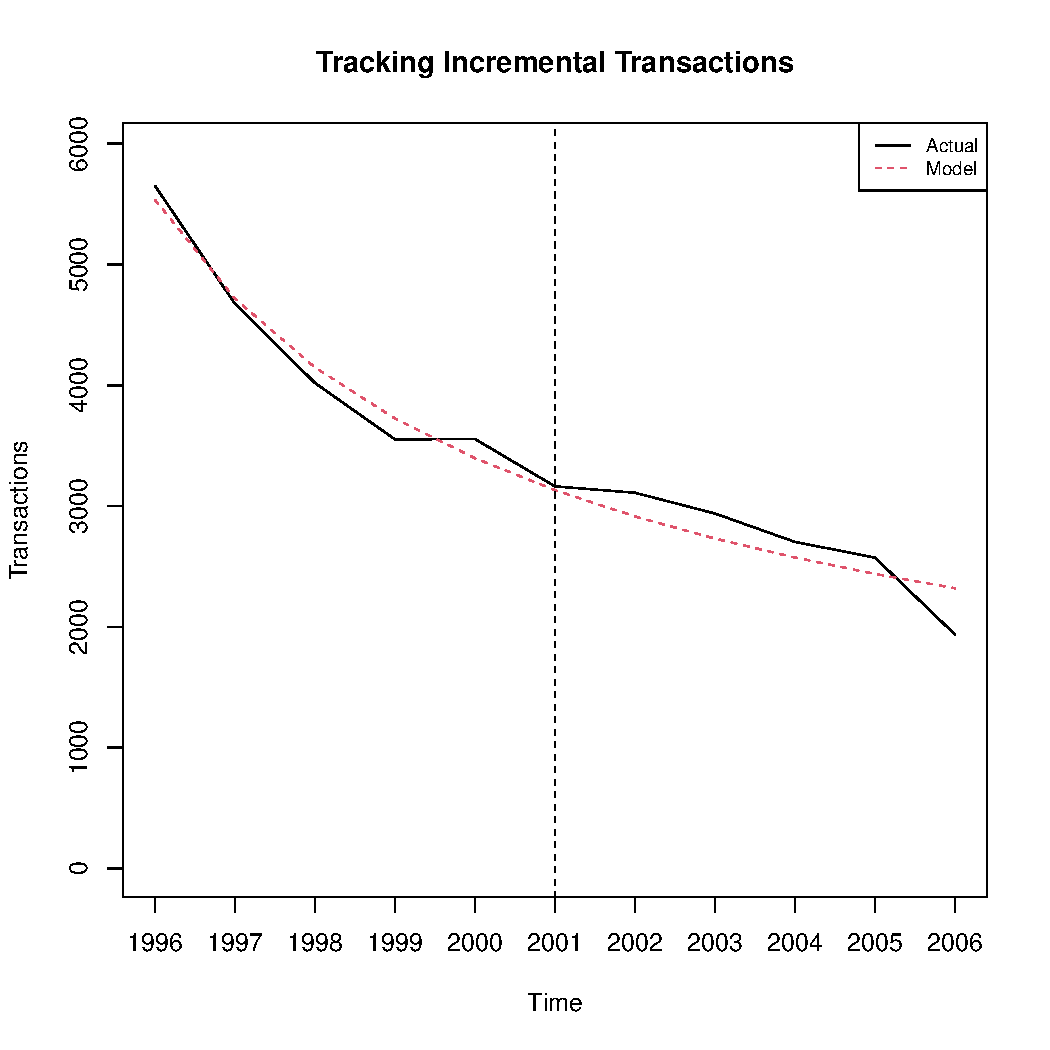
\includegraphics[width=0.6\textwidth]{figure/bgbbTrackingInc}
  \caption{Actual vs. expected incremental purchasing behaviour.}\label{fig:bgbbTrackingInc}
  \end{center}
\end{figure}

Figure \ref{fig:bgbbTrackingInc} shows remarkable fit, but we can
smooth it out for a cleaner graph by making it cumulative (as shown in
figure \ref{fig:bgbbTrackingCum}).

\begin{knitrout}\small
\definecolor{shadecolor}{rgb}{0.969, 0.969, 0.969}\color{fgcolor}\begin{kframe}
\begin{alltt}
\hlstd{cum.track.data} \hlkwb{<-} \hlkwd{cumsum}\hlstd{(inc.track.data)}
\hlkwd{pdf}\hlstd{(}\hlkwc{file} \hlstd{=} \hlstr{'figure/bgbbTrackingCum.pdf'}\hlstd{)}
\hlstd{cum.tracking} \hlkwb{<-} \hlkwd{bgbb.PlotTrackingCum}\hlstd{(params, rf.matrix, cum.track.data,}
                                     \hlkwc{xticklab} \hlstd{= xtickmarks)}
\hlkwd{dev.off}\hlstd{()}
\end{alltt}
\begin{verbatim}
# pdf 
#   2
\end{verbatim}
\begin{alltt}
\hlkwd{rownames}\hlstd{(cum.tracking)} \hlkwb{<-} \hlkwd{c}\hlstd{(}\hlstr{"act"}\hlstd{,} \hlstr{"exp"}\hlstd{)}
\hlstd{cum.tracking}
\end{alltt}
\begin{verbatim}
#         [,1]     [,2]     [,3]     [,4]     [,5]     [,6]     [,7]     [,8]
# act 5652.000 10326.00 14345.00 17897.00 21452.00 24615.00 27725.00 30663.00
# exp 5535.833 10252.89 14400.51 18125.18 21521.07 24652.71 27566.49 30296.97
#        [,9]    [,10]    [,11]
# act 33366.0 35939.00 37875.00
# exp 32870.7 35308.56 37627.29
\end{verbatim}
\end{kframe}
\end{knitrout}

\begin{figure}
  \begin{center}
  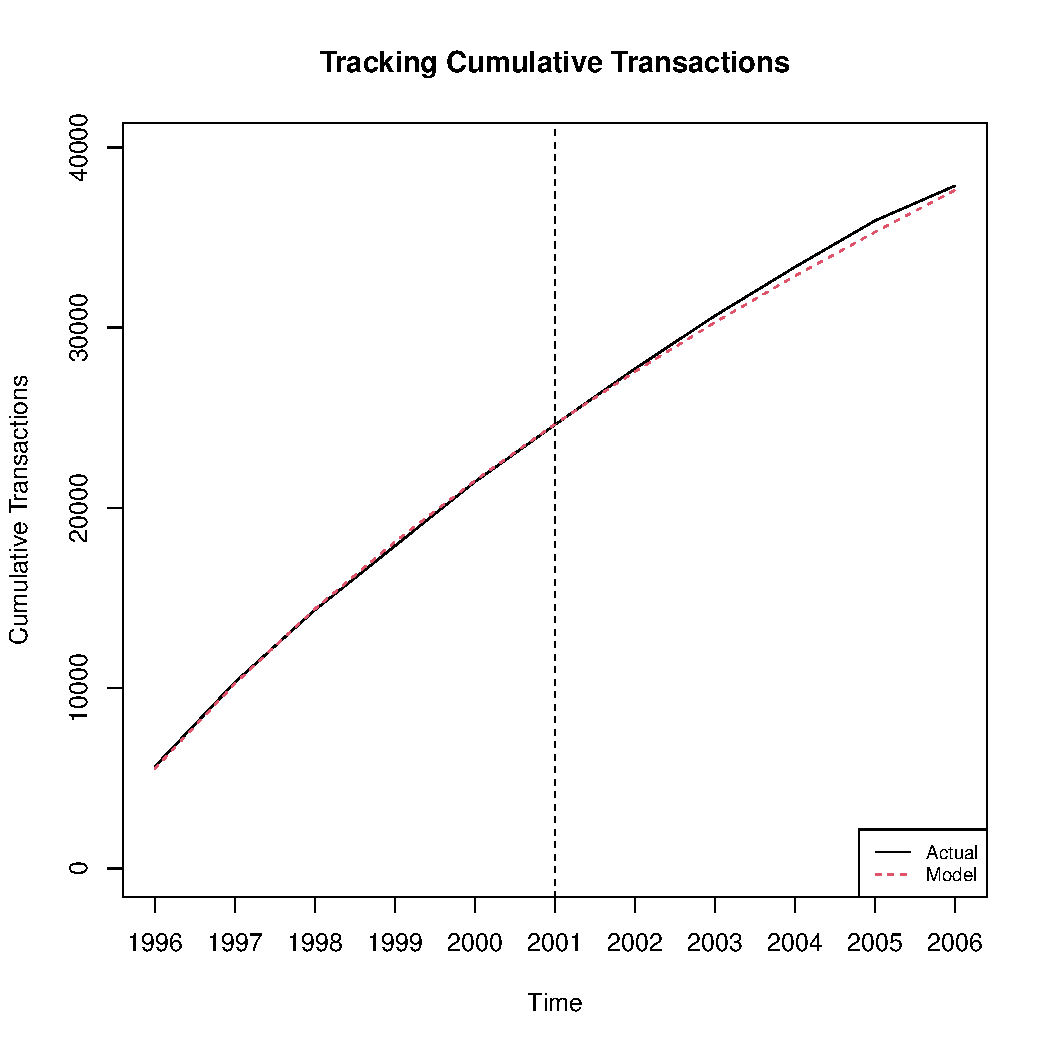
\includegraphics[width=0.6\textwidth]{figure/bgbbTrackingCum}
  \caption{Actual vs. expected cumulative purchasing behaviour.}\label{fig:bgbbTrackingCum}
  \end{center}
\end{figure}

\section{Further analysis}

The package functionality I highlighted above is just a starting point
for working with these models. There are additional tools, such as
functions for discounted expected residual transactions (the present
value of the remaining transactions we expect a customer to make) and
an implementation of the gamma-gamma spend model, which may come in
useful for customer analysis. Hopefully you now have an idea of how to
start working with the BTYD package - from here, you should be able to
use the package's additional functions, and may even want to implement
some of your own. Enjoy!

\clearpage

\section*{References}

\setlength{\parindent}{0pt} \setlength{\parskip}{1ex plus 0.2ex minus 0.2ex}

Fader, Peter S., and Bruce G.S. Hardie. ``A Note on Deriving the Pareto/NBD Model and Related Expressions.''
November. 2005. Web.\\ \href{http://www.brucehardie.com/notes/008/}{\textless http://www.brucehardie.com/notes/008/\textgreater}

Fader, Peter S., Bruce G.S. Hardie, and Jen
Shang. ``Customer-Base Analysis in a Discrete-Time Noncontractual Setting.'' \emph{Marketing Science}, \textbf{29(6)},
pp. 1086-1108. 2010. INFORMS.\\ \href{http://www.brucehardie.com/papers/020/}{\textless http://www.brucehardie.com/papers/020/\textgreater}

Fader, Peter S., Hardie, Bruce G.S., and Lee,
Ka Lok. ````Counting Your Customers'' the Easy Way: An Alternative to the Pareto/NBD Model.'' \emph{Marketing Science}, \textbf{24(2)},
pp. 275-284. 2005. INFORMS.\\ \href{http://brucehardie.com/papers/018/}{\textless http://brucehardie.com/papers/018/\textgreater}


\end{document}

